%%%%%%%%%%%%%%%%%%%%%%%%%%%%%%%%%%%%%%%%%%%%%%%%%%%%%%%%%%%%%%%%%%%%
%% texplate.tex
%% NOVA thesis document template
%%
%% This work is licensed under the 
%% Creative Commons Attribution-NonCommercial 4.0 International License. 
%% To view a copy of this license, 
%% visit http://creativecommons.org/licenses/by-nc/4.0/.
%%
%% Version 2017/07/26 [4.1.2]
%% Departamento de Informática
%% Faculdade de Ciências e Tecnologia
%% Universidade NOVA de Lisboa
%%
%% BUGS and SUGGESTIONS: please submit an issue at the project web page
%%      at: https://github.com/joaomlourenco/novathesis/
%%
%% HELP: please ask for help at the NOVAthesis google group at
%%          https://groups.google.com/forum/#!forum/novathesis
%%      or at the facebook page
%%          https://www.facebook.com/groups/novathesis/
%%
%% Authors / Contributors:
%%      - João Lourenço <joao.lourenco@fct.unl.pt>
%%      - Bruno Candeias <b.candeias@campus.fct.unl.pt>
%%
%% DONATIONS:
%%     If you think this templatze really helped you while writing your thesis,
%%     think about doing a small donation. Just access the website 
%%     https://github.com/joaomlourenco/novathesis/
%%     and click in the “Donation” link.
%%     I'll keep a list thanking to all the identified donors that identify
%%     themselves in the “*Add special instructions to the seller:*” box.
%%%%%%%%%%%%%%%%%%%%%%%%%%%%%%%%%%%%%%%%%%%%%%%%%%%%%%%%%%%%%%%%%%%%%

% The default option marked with (*)
\documentclass[
  docdegree=msc,        % phd(*), phdplan, phdprop, msc, mscplan, bsc
  school=nova/fct,      % nova/fct(*), nova/fcsh, nova/ims, ul/ist, ul/fc
  lang=en,              % en(*), fr, it, pt
  coverlang=pt,         % defaults to main language
  copyrightlang=pt,     % defaults to main language
  fontstyle=kpfonts,    % baskervaldx bookman charter ebgaramond fbb fourier garamond
                        % heuristica kpfonts(*) libertine mathpazo1 mathpazo2 newcent
                        % newpx newtx 
  chapstyle=elegant,    % bianchi bluebox brotherton dash default elegant(*) ell ger 
                        % hansen ist jenor lyhne madsen pedersen veelo vz14 vz34 vz43
  otherlistsat=front,   % front(*), back
  aftercover=false,     % false=don't true=include the aftercover file (even if exists)
  linkscolor=darkblue,  % darkblue, black (Set to 'black' for PRINTING)
  printcommittee=true,  % set to 'false' from submitted versins who should not have 
                        % the list of committee memebers
  spine=false,          % (Set to 'true' for PRINTING the book spine)
  cdcover=false,         % (Set to 'true' for PRINTING the CD cover)
  biblatex={            % Options for biblatex (see biblatex documentation)
    %%%%%%%%%%%%%%%%%%%%%%%%%%%%%
    %%% uncomment for 'apa' like citations
    % backend=biber,    % must use biber as the backend (and not bibtex)
    % natbib=true,      % compatiblity with natbib (use \cite{…} or \citep{…})
    % style=apa,        % APA style
    % maxcitenames=2,   % use at most two names in citation
    %%%%%%%%%%%%%%%%%%%%%%%%%%%%%
    %%% uncomment for 'numeric-by-order-of-citation' like citations
    % backend=bibtex,     % use bibtex if possible
    % style=numeric-comp, % numeric(*), alphabetic, authoryear, bwl-FU
    % sortcites=true,     % If numeric, sort cites by crescent order
    % sorting=none,       % none, nyt(*), ynt
    %%%%%%%%%%%%%%%%%%%%%%%%%%%%%
    %%% uncomment for 'numeric-by-order-of-citation' like citations
    backend=bibtex,     % use bibtex if possible
    style=numeric-comp, % numeric(*), alphabetic, authoryear, bwl-FU
    sortcites=true,     % If numeric, sort cites by crescent order
    sorting=nyt,        % none, nyt(*), ynt
    %%%%%%%%%%%%%%%%%%%%%%%%%%%%%
    %%% uncomment for 'numeric-by-order-of-citation' like citations
    % backend=bibtex,   % use bibtex if possible
    % style=alphabetic, % numeric(*), alphabetic, authoryear, bwl-FU
    % sorting=nyt,      % none, nyt(*), ynt
    %%%%%%%%%%%%%%%%%%%%%%%%%%%%%
    %%% other options for biblatex
    maxbibnames=99,     % Never use 'et al' in the bibliography
    giveninits=true,    % render all first and middle names as initials
    hyperref=true       % Hyperlinks in citations: true(*) false
  },
  memoir={              % See the 'memoir' documentation
    % showtrims,          % DEBUG
    a4paper,            % the paper size/format
    11pt,               % 10pt, 11pt(*), 12pt
    final,              % draft, final  <= Replace 'draft' with 'final' in final version
  },
  media=screen,         % screen(*), paper
          % behavior to be defined in school options based in "\novathesis@opt@media"
          % definitions for screen: left and right margins are equal, colored links
          % definitions for paper: left and right margins are different, black links
]{novathesis}



%%============================================================
%%
%%  BEGINING OF USER COSTUMIZATION
%%
%%============================================================


%------------------------------------------------------------------
% Additional packages you may want to use (comment those not needed)
%------------------------------------------------------------------

%% VERY IMPORTANT
\usepackage{booktabs}    % Beautiful simple tables
\usepackage{paralist}    % To enable customizble enumerates

%% IMPORTANT (consider removing/commenting)
%\usepackage{colortbl}    % Use colors in background of table cells
\usepackage[textsize=footnotesize]{todonotes}  % To register TODO notes in the text
\setlength{\marginparwidth}{3.25cm}



%% FOR DEMO PURPOSES ONLY --- TO BE REMOVED by final users
\usepackage{lipsum}

%% MY PACKAGES

\usepackage{enumitem}


%------------------------------------------------------------------
% Costumization of some packages
%------------------------------------------------------------------

% Where to look for figures
% \prependtographicspath{{some-folder-here}}

% Setup of listings, for more information check the 'listings' package manual
% \lstset{
%     captionpos=t,
%     basicstyle={\ttfamily\footnotesize},
%     numbers=left,
%     numberstyle={\ttfamily\tiny},
%     tabsize=2,
%     language=Java,
%     float,
%     frame=single,
% }




%%============================================================
% For costumization,
%        see file 'nova-thesis/Schools/*/*/defaults.clo'
%        and file 'nova-thesis/lang-text.clo'
% You may override here any of the values defined there
% e.g.
% \majorfield[pt]={Engenharia Biomédica}
% \majorfield[en]={Biomedical Engineering}
% \thesiscover[msc,front]={cover-megi-nova-ims}
% \thesiscover[msc,front]={cover-mgi-nova-ims}
%%============================================================

% Title of the dissertation/thesis
% USe "\\" to break the title into two or more lines
% \let\oldtitle=\title
% \makeatletter
% \renewcommand{\title}[2][]{%
%   \ifthenelse{\equal{#1}{}}%
%     {\newcommand{\covertitle}{#2}}%
%     {\newcommand{\covertitle}{#1}}%
%   \let\title=\oldtitle
%   \title{#2}
% }
% \makeatother

\title[An effective Pest Monitoring System for outdoor farms]{An effective Pest Monitoring System for outdoor farms}
\subtitle{Science is beautiful}

% Autor
% use [f] for female and [m] for male
\authorname[m]{Hugo Gonçalves Pereira António}{Hugo António}
\authordegree{Master of Science}

% Date
\datemonth{July}
\dateyear{2018}


% Advisers
% use "\\&" if necessary to break the lines in the apprpriate place
% use [f] for female and [m] for male
\adviser[m]{João Carlos Gomes Moura Pires}{Auxiliary Professor}{\\& NOVA University of Lisbon} 
% you may use "\newline" to force a new line
% \adviser[m]{John Doe Male Adviser Name}{Associate\\& Professor}{Some University Somewhere}
% \adviser[m]{John Doe Third Adviser Name}{Associate\\& Professor}{Some University Somewhere}


% Co-Advisers (maximum of 9)
% use [f] for female and [m] for male
\coadviser[m]{Carlos Augusto Viegas Damásio}{Auxiliary Professor}{NOVA University of Lisbon}
% \coadviser[f]{[Nome da co-orientadora 2]}{[Profª.\ Auxiliar]}{[Universidade Nova de Lisboa]}


% committee (maximum of 9 elements)
% Use [c] for chair, [r] for raporteurs, [a] for advisers, [m] or nothing for remaining members
% Chair of the committee
\committee[c,m]{Name of the committee chairperson}
% Main raporteurs
\committee[r,f]{Name of a raporteur}
\committee[r,f]{Name of another raporteur}
% Advisers
\committee[a,f]{Name of an adviser}
\committee[a,f]{Name of another adviser}
% Other members of the committee - include the Adviser in this list
\committee[m,m]{Another member of the committee}
\committee[m,f]{Yet another member of the committee}

%%------------------------------------------------------------
%% All the names inside braces below sould correspond to a file
%%     with extension ".tex" and located in the "Chapters" folder
%%------------------------------------------------------------

% Dedicatory text. Will only be considered for final documents,
% i.e., "bsc", "msc" and "phd", otherwise, it will be silently ignored
%\dedicatoryfile{dedicatory}

% Acknowledgments text. Will only be considered for final documents,
% i.e., "bsc", "msc" and "phd", otherwise, it will be silently ignored
%\acknowledgementsfile{acknowledgements}


% \quotefile{quote}    % Quote
\abstractfile[pt]{abstract-pt}  % Abstract in Portuguese
\abstractfile[en]{abstract-en}  % Abstract in English
\abstractfile[fr]{abstract-fr}  % Abstract in French
\glossaryfile{glossary}
\setglossarystyle{super}
\acronymsfile{acronyms}

% definition of the second cover, to be printed before the copyright (to serve FCSH-NOVA)
\aftercoverfile{aftercover-nova-ims}


% The Table of Contents is always printed.
% The other lists below may be commented and omitted.
\addlisttofrontmatter{\listoffigures}  % The List of Figures. Comment to omit.
\addlisttofrontmatter{\listoftables}   % The List of Tables. Comment to omit.
\addlisttofrontmatter{\lstlistoflistings}  % The List of Code Listings. Comment to omit.
\addlisttofrontmatter{\glsnogroupskiptrue\setlength{\glsdescwidth}{0.8\textwidth}\printnoidxglossaries}  % The Glossary and List of Acrnonyms


% Text chapters
% syntax: \chapterfile{file}
\chapterfile{chapter1}
\chapterfile{chapter2}
\chapterfile{chapter3}
% \chapterfile{chapter4}


% Text appendixes
% sintax: \appendixfile{file}
% Comment if not needed
% \appendixfile{appendix1}
% \appendixfile{appendix2}
% \annexfile{annex1}
% \annexfile{annex2}


% BibTeX bibiography files. Can be used multiple times with a single file nae each time.
\addbibfile{bibliography.bib}



%%==== DANGER ==== DANGER ==== DANGER ==== DANGER ==== DANGER ====
%%==== DANGER ==== DANGER ==== DANGER ==== DANGER ==== DANGER ====
%%==== DANGER ==== DANGER ==== DANGER ==== DANGER ==== DANGER ====
%%
%%  END OF USER COSTUMIZAITON
%% Please do not change below this point!!! :)
%%
%%==== DANGER ==== DANGER ==== DANGER ==== DANGER ==== DANGER ====
%%==== DANGER ==== DANGER ==== DANGER ==== DANGER ==== DANGER ====
%%==== DANGER ==== DANGER ==== DANGER ==== DANGER ==== DANGER ====


%% Begining of document
\begin{document}

%%%%%%%%%%%%%%%%%%%%%%%%%%%%%%%%%%%%%%%%%%%%%%%%%%%%%%%%%%%%%%
\thesisfrontmatter  % Before the main text (TOC, etc)
%%%%%%%%%%%%%%%%%%%%%%%%%%%%%%%%%%%%%%%%%%%%%%%%%%%%%%%%%%%%%%
\printcoverpage    % The cover page
\printaftercover
\printcopyright    % Print the copyright page (will only be printed if adequate for the document type)
\printdedicatory  % Print the dedicatory (will only be printed if adequate for the document type)
\printacknowledgements  % Print the acknowledgments (will only be printed if adequate for the document type)
\printquote        % Print the quote (if file exists and is adequate for the document type)
\printabstract    % Print abstracts (in PT and EN). The abstract in the document main language will
                  % be printed first, the abstract in the foreign language will be printed second
\printtoc         % Always print the table of contents
\printotherlists   % If option 'otherlistsat=front', print other lists of contents according
                  % to instructions given above, otherwise do nothing


%%%%%%%%%%%%%%%%%%%%%%%%%%%%%%%%%%%%%%%%%%%%%%%%%%%%%%%%%%%%%%
\thesismainmatter  % The main text
%%%%%%%%%%%%%%%%%%%%%%%%%%%%%%%%%%%%%%%%%%%%%%%%%%%%%%%%%%%%%%
\printchapthers    % Print document chapters
\printbib    % Print the bibliography
% \printotherlists   % Alternative location to print the other lists (if you uncomment this one, comment the other one above)
\printotherlists   % If option 'otherlistsat=back', print other lists of contents according to instructions given above, otherwise do nothing
\printappendixes  % Print appendixes, if any!
\printannexes  % Print appendixes, if any!
\printbackcoverpage
%%%%%%%%%%%%%%%%%%%%%%%%%%%%%%%%%%%%%%%%%%%%%%%%%%%%%%%%%%%%%%
%% End of document
%%%%%%%%%%%%%%%%%%%%%%%%%%%%%%%%%%%%%%%%%%%%%%%%%%%%%%%%%%%%%%
\end{document}


%%%%%%%%%%%%%%%%%%%%%%%%%%%%%%%%%%%%%%%%%%%%%%%%%%%%%%%%%%%%%%
%% Includes For Texpad
%%%%%%%%%%%%%%%%%%%%%%%%%%%%%%%%%%%%%%%%%%%%%%%%%%%%%%%%%%%%%%
%!TEX root = ../template.tex
%%%%%%%%%%%%%%%%%%%%%%%%%%%%%%%%%%%%%%%%%%%%%%%%%%%%%%%%%%%%%%%%%%%%
%% abstrac-pt.tex
%% NOVA thesis document file
%%
%% Abstract in Portuguese
%%%%%%%%%%%%%%%%%%%%%%%%%%%%%%%%%%%%%%%%%%%%%%%%%%%%%%%%%%%%%%%%%%%%

Culturas agrícolas são alvo de inúmeras pragas e mudanças climatéricas que podem causar danos económicos. É essencial recolher estes dados e prever potenciais ocorrências de  problemas nestas culturas.

Para solucionar um método de recolha de dados inadequado, cadernos de campo, esta dissertação visa desenvolver uma framework na forma de aplicação que permita registar dados e eventos na plantação, geovisualizar o estado das plantas e monitorizar as pragas inimigas da cultura plantada.

Desde estações meteorológicas, sensores de solo e observações biológicas de pragas, dados vão ser coletados do campo de cultivo para o servidor e devolvidos ao utilizador/agricultor na forma de uma visualização digital interativa: Mapas de risco. Todos os dados coletados devem ser geo-referenciados e serão obtidos com dispositivos móveis (smartphones) e/ou sensores \emph{in situ}, documentados com fotografias, vídeos e texto sempre que necessário. Esta dissertação descreve e apresenta uma \emph{framework} que emprega a metodologia da Agricultura de Previsão que é destinada a recolher informação e calcular métricas relevantes sobre os dados de diferentes fontes sensoriais de uma forma escalável.

A solução apresentada neste documento deve auxiliar agricultores na tomada de melhores decisões ao gerir as suas propriedades agrícolas, ajudar a documentar o comportamento de algumas espécies de insetos e reduzir a perda de produção dos parceiros do grupo operacional FitoAgro. 

% Palavras-chave do resumo em Português
\begin{keywords}
Pragas, mudanças climatéricas, recolha de dados, cadernos de campo, geovisualização, framework, estações meteorológicas, dispositivos móveis, sensores, observações biológicas, agricultura de precisão, FitoAgro \ldots
\end{keywords}
% to add an extra black line

%!TEX root = ../template.tex
%%%%%%%%%%%%%%%%%%%%%%%%%%%%%%%%%%%%%%%%%%%%%%%%%%%%%%%%%%%%%%%%%%%%
%% abstrac-en.tex
%% NOVA thesis document file
%%
%% Abstract in English
%%%%%%%%%%%%%%%%%%%%%%%%%%%%%%%%%%%%%%%%%%%%%%%%%%%%%%%%%%%%%%%%%%%%
Crops are subject to numerous pests and weather variables that may cause significant economic damage. It is essential to aggregate this data and forecast the potential occurrence of the major problems in these crops. 

To fix an inadequate data collection process, the goal of this dissertation is the development of a framework in the form of platform for data/event registering and geovisualization of plant status and pest monitoring.

Ranging from weather stations, soil sensors and pest biological observations; data will be collected from the field to the server and given back to the user/farmer in the form of a rich digital visualization: Risk Maps. All the data collected shall be geo-referenced and will be obtained with mobile devices or sensors \emph{in-situ}, documented with photos, videos and text whenever needed.
This thesis describes and presents a fully working framework that employs the methodology from Precision Agriculture that is able to collect data and compute metrics from the several sources of information available, in a scalable way.

The solution presented in this work will empower farmers to make better decisions when managing their properties, help documenting specific species behaviour and reduce yield loss for the partners in the FitoAgro operational group.

% Palavras-chave do resumo em Inglês
\begin{keywords}
Framework, Data Collection, Precision Agriculture, Geovisualization, mobile devices, sensors, Web Application, Pest Monitoring, Risk Maps, FitoAgro.
\end{keywords} 

\include{Chapters/dedicatory}
\include{Chapters/acknowledgements}
%!TEX root = ../template.tex
%%%%%%%%%%%%%%%%%%%%%%%%%%%%%%%%%%%%%%%%%%%%%%%%%%%%%%%%%%%%%%%%%%%
%% chapter1.tex
%% NOVA thesis document file
%%
%% Chapter with introduciton
%%%%%%%%%%%%%%%%%%%%%%%%%%%%%%%%%%%%%%%%%%%%%%%%%%%%%%%%%%%%%%%%%%%
\newcommand{\novathesis}{\emph{novathesis}}
\newcommand{\novathesisclass}{\texttt{novathesis.cls}}


\chapter{Introduction}
\label{cha:introduction}

\section{Motivation and context} %%%%%%%%%%%%%%%%%%%%%%%%%%%%%%%%
\label{sec:motivation_and_content}

Throughout the history of humanity, plant pests and diseases have been numerous times responsible for significant losses in society. Effects range from starvation, extinction of natural resources, negative impact on national/international resources or even deaths in a population.

Nowadays, pests and diseases do not present such threats but still constitute a relevant problem since they result in substantial losses to farmers by reducing the value of their products: yield loss, as studied in \cite{Kamilaris2017}\cite{Walker1983}. To minimize yield loss, there are two main approaches when handling plant pests and diseases: \emph{Prevention and Treatment}.

Prevention is based on prediction models, field records or general management tactics that are applied before the plants are actually infected \cite{StuartB.Hill}. Treatment, on the other hand, is all about deploying active substances to fight the already present disease. Prevention is obviously the preferable option when handling pest control since it represents no yield loss and no chemicals are used.

This dissertation, while focusing on prevention, proposes a framework/methodology for data collection and visualization of outdoor farming fields. This means tracking the growth of the plants, the location and intensity of the pest, soil information and climatic conditions. Several pests will be studied, but more than a system to fight specific pests (or pests in specific cultures), a framework that may be used to study the connections between Botany (the cultivated plant species), Entomology (parasite species), soil and climatic conditions will be created. 

During the development of this dissertation, the \emph{Fitoagro} project will be used as a case study of the methodology. \emph{Fitoagro}, as an Operational Group, consists of several partners with a common interest in a specific, practical innovation project: Pest Monitoring for the Apple and Pear Cultures in West Portugal. The people involved in the Operational Group come from a diverse combination of practical and scientific backgrounds (farmers, scientists, agri-business and others). Below are listed the main partners of the Fitoagro project.

\begin{description}
	\item [COTHN] Centro Operativo e Tecnológico Hortofrutícola Nacional
	\item [FCT/UNL] Faculdade de Ciências e Tecnologia da Universidade Nova de Lisboa
	\item [ISA] Instituto Superior de Agronomia
	\item [ESAS] Escola Superior Agrária de Santarém
	\item [ESACB] Escola Superior Agrária de Castelo Branco
\end{description}

Other entities such as agricultural cooperatives will also directly contribute as associates of the COTHN national entity, mainly in the data-collection process and the study of the biological species present in their very own farming fields. These above-listed organisations work together on specific and practical solutions to the following emerging pests (harmful ectoparasites):

\begin{enumerate}
	\item \textit{Dasineura pyri (Bouché)}
	\item \textit{Aphanostigma pyri}
	\item \textit{Stemphylium vesicarium}
	\item \textit{Pseudococcus viburni / Planococcus ficus}
\end{enumerate}

To successfully study a species, a significant amount of data is needed. That being said, if the current farming season brings new pest species with a decent number of samples, they will be considered to the study.

With features ranging from data collection to a visual monitoring system, the FitoAgro system will be able to visually empower producers and farmers to make better decisions when protecting their assets from pests and diseases. A couple of research questions waiting to be answered are "Can we detect a geographic pattern in a pest's behaviour?" or "Can the data collection process of pest occurrences be automated?". 

% section motivation_and_content (end) %%%%%%%%%%%%%%%%%%%%%%%%%%%%%%%%


\section{Problem} % (fold) %%%%%%%%%%%%%%%%%%%%%%%%%%%%%%%%
\label{sec:problem}

\subsection{Historical background and World Population Growth} % (fold)
\label{subsec:historical_background}

The first agricultural revolution came along during the advent of increased mechanization, from 1900 to 1930. Each farmer produced enough food to feed about 26 people during this time \cite{DongoskiRob}.
%
The 1990s prompted the Green Revolution with new methods of genetic modification, which led to each farmer feeding about 155 people.
%
It is expected that by 2050, the global population will reach about 9.6 billion \cite{DESA2015}, and food production must effectively double from current levels in order to feed every mouth. With new technological advancements in the agricultural revolution of precision farming, each farmer is expected be able to feed 265 people on the same acreage \cite{DongoskiRob}.

Digital agriculture is widely recognized as the third great revolution of modern agriculture. The introduction and implementation of mechanization (1900 to 1930) and genetic modification (1990 to 2005) are referred to as Ag 1.0 and Ag 2.0 respectively. Both revolutions drove efficiency, yield and profitability to levels previously unattainable, and are now conventional in developed countries across the world.

While Ag 1.0 and Ag 2.0 definitely drove significant changes in agriculture, Ag 3.0 will be the most transformative and disruptive, not only on the farm, but across the entire agriculture and food value chain \cite{Lewis&ClarkVentures}.

\subsection{The ever going study of Pest}
\label{subsec:evergoing_study_pest}

A Pest is any plant or animal detrimental to humans or human concerns including crops, livestock, and forestry. In its broadest sense, a pest is a competitor of humanity. Pests are usually categorized by taxon. Different taxonomies are usually studied by different branches of Biology. 

The term "plant pest" has a specific definition in terms of the \textit{International Plant Protection Convention} and phytosanitary measures worldwide. A pest is any species, strain or biotype of plant, animal, or pathogenic agent injurious to plants or plant products. 

Pest and disease study is, obviously, a continuous field of study since human interaction keeps disturbing nature's balance, which eventually leads to mutations, migrations, species. Plant pests keep developing resistances against active substances used in the fields (pesticides). Pest species evolve pesticide resistance via natural selection: the most resistant specimens survive and pass their genetic traits to their offspring. Although the evolution of pesticide resistance is usually discussed as a result of pesticide use, it is important to keep in mind that pest populations can also adapt to non-chemical methods of control.

Speciation (repeated formation of new species) leads to a hierarchical structure of the same species that developed specific traits for each culture it threatens. According to \cite{Sharma2014} pest life cycles are also changing so their first seasonal appearance is gradually evolving over time. All the above-mentioned factors contribute to the idea that pest control is still a problem, and Nature makes sure of that. Proper models have to constantly be built for new species, new traits, different conditions etc. 


\subsection{Spreadsheets}

Even though the problems mentioned in \ref{subsec:historical_background} and \ref{subsec:evergoing_study_pest} stand as important, there is a more practical and urgent problem.

Technological advances offer tools to farming management tools, mostly by providing a data collection system: weather and Soil stations display their readings on proprietary web interfaces. Biological Measurements however are tracked using paper spreadsheets which are afterwards uploaded to a document-sharing service like \textit{Google Drive}. While acceptable for small farms and direct measurement analysis ("Is the temperature above 40ºC in the field?"), it is hard to build logic that combines weather, soil and enemy-tracking data that can sucessfully draw conclusions.

These paper spreadsheets are used \emph{in-situ} and track phenological stages of the crop, enemy observations, dates of phytopharmaceutical product applications and production system data. An enemy observation spreadsheet for a single farming field is available in \ref{fig:spreadsheet}. On the spreadsheet, the \textit{Barrocalvo} farming field is sampled 4 times (dates on the table header) on different phenological stages for a specific enemy: Aphanostigma pyri. A1-A10 are the ten randomly selected trees being monitored. For each tree, 3 adhesive tapes are placed on the trunk(T) and 2 branches(P1 and P2). On the date column, zeros and ones are the counts for the enemy(insects) on the traps (adhesive tapes). 

Figure \ref{fig:spreadsheet} also shows a perfect example of how irregular the registering method is: on the 11th of April, in the trunk of the tree number seven, it is not clear how many enemies were tracked.

\begin{figure}[htbp]
  \centering
  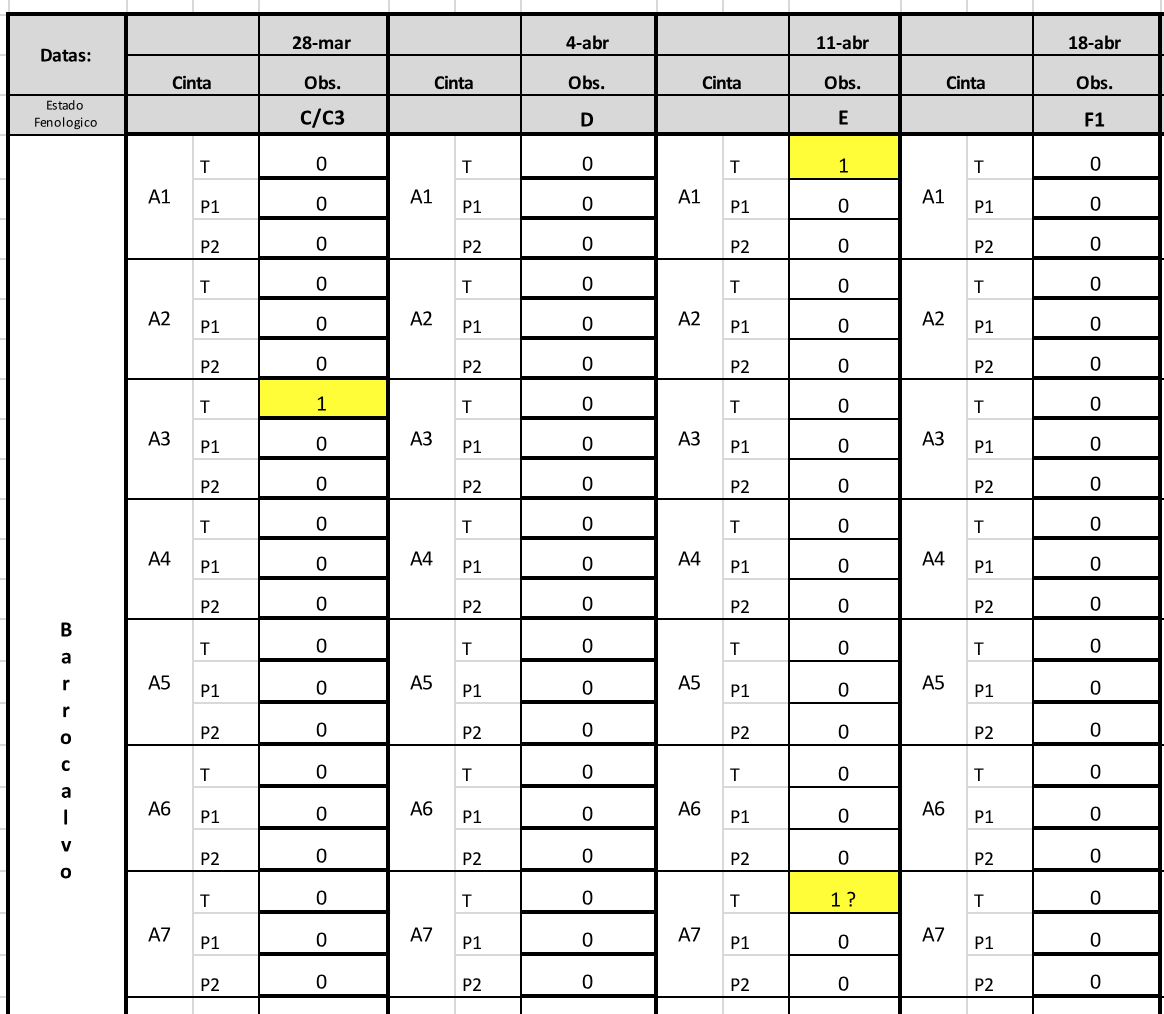
\includegraphics[width=0.85\linewidth]{spreadsheet}
  \caption{A sample from the collaborative spreadsheet for the \textit{Barrocalvo} farming field (FitoAgro project)}
  \label{fig:spreadsheet}
\end{figure}

More details on the use of these field-notebooks is available in chapter \ref{cha:problem}.

\section{Objectives} % (fold) %%%%%%%%%%%%%%%%%%%%%%%%%%%%%%%%
\label{sec:objective}

\subsection{Precision Agriculture}
\label{sec:precision_agriculture}

Precision Agriculture(PA) , Satellite Farming or Site-specific crop management (SSCM) is a key-component  of the third wave of modern agricultural revolutions (Ag 3.0). In it's essence, it is a farming management concept based on observing, measuring and responding to inter and intra-field variability in crops. Its main goal is to provide a decision support system for a whole farm management in order to optimize returns on inputs and, most importantly, preserving resources.

The basic principle of precision farming is an exact positional controlling of fertilisation, growth levels, pest presence, risk estimate or any other relevant key-performance indicator with the accuracy of a few meters. The whole process requires a big amount of data to be collected which enables the control of the management process. The better the data collection method, the more resolution data will have, which allows for better conclusions to be taken. Studies conducted on Precision Agriculture as \cite{Khanal2017} \cite{Talavera2017} \cite{Kruize2016} \cite{Culibrina2015} \cite{Jawad2017} \cite{Resu2015} \cite{Alam2014} \cite{JointResearchCentreJRCoftheEuropeanCommission2014} \cite{Mohanraj2016} \cite{Sankaran2010} \cite{Nip2003} show different approaches in data collection with different resolutions. Most of the recent efforts are incorporating \emph{IOT} (Internet of Things) in the agricultural domain leading to a plant-level analysis of the field. Most of the described sensor meshes, ul have high costs and therefore are not analised in chapter \ref{cha:state_of_the_art} since they do not present a reasonable choice for medium-scale independent producers such as the cooperatives from the FitoAgro project mentioned in \ref{sec:motivation_and_content}.

From the works listed above, Precision Farming is usually divided into the following steps:

\begin{description}
\item [Data Collection] Inter field systems collect data with a field-level of resolution. Increasing the number of sources provides a smaller scale analysis. Geolocating data sources enables the farmer to read a map of his property (henceforth called soil map) with the most important crop variables.
\item [Variables] The data collected can measure different things. Usually, climatic conditions (hail, drought, rain, etc.), soils (texture, depth, nitrogen levels), cropping practices (no-till farming), weeds and disease. Permanent indicators as weather stations, provide information about the main environmental constants. Point indicators allow them to track a crop’s status, i.e., to see whether diseases are developing, if the crop is suffering from water stress, nitrogen stress, or lodging, whether it has been damaged by ice and so on. This information may come from weather stations and other sensors (soil electrical resistivity, detection with the naked eye, satellite imagery, etc.). Soil resistivity measurements combined with soil analysis make it possible to measure moisture content. Soil resistivity is also a relatively simple and cheap measurement.
\item [Strategies] Once with soil maps, Strategies can be either predictive (Predictive Approach), where   based on history and static features of the field, the farmer takes decisions. The Control Approach, on the other hand, collects data regularly during the crop cycle to provide a better temporal resolution. Decisions may be based on decision-support models and/or the farmer.
\item [Implementing practices] If some decisions are to be trusted to an algorithm, Variable Rate Technology can help to administer variable rates of pesticides(biological or chemical), nutrients, water, etc. through Variable Rate Application (VRA). Map Based and Sensor Based VRA present two very different paths.
\end{description}	

These simple four steps present a methodology for the continuous management of the farming field.

The main objective of this dissertation is to combine the methodology from Precision Agriculture with Pest Control strategies and build a framework that geographically maps important variables of a farming field.

Available options for Data Collection are studied in detail in chapter \ref{sec:state_of_the_art_data}. They include data sources such as as soil, weather and biological readings from different sources regarding: cost, efficiency, resolution, limitations while focusing on the needs of the Pest study. This framework will enable the building of regional risk maps (geographic likelihood of yield loss) for any outdoor farming field. For the end-user of the framework, farmers, some visualization techniques will be applied to ease-out farm management tasks.

The resulting framework will be available through a mobile interface and should empower farmers to make better decisions while managing their property by displaying sensor data in a map visualization adjusted to the agricultural domain. 

% section problem_and_objective (end)

\section{Major Contributions} % (fold) %%%%%%%%%%%%%%%%%%%%%%%%%%%%%%%%
\label{sec:contributions}

\subsection{State of the Art as a Review of Recent Efforts}
\label{sec:review_recent_efforts}

The State of the Art presents a good contribution itself. By organising and cathegorising different techniques by data source it is expected to achieve a detailed analysis of the recent trends in outdoor data collection as well as pest control methodologies.

\subsection{A framework for data collection and visualization of a farming field}
\label{sec:digital_mapping_framework}

Farming fields have, by default, ideal conditions for the development of life. That's why they are farming fields. Plants, as the farmer's objective, greatly benefit from this. The problem is that parasite species may also be present, parasitizing whatever plant species is being cultivated in the field.

This creates both a difficult problem for the farmer but also an interesting problem for the study of specific species.

By capturing as many field variables as possible, a geographic model of the farming field can be built. Sensoring organic growth levels for both (plant and pest) species as well as climatic variables may empower farmers to make better decisions on their farming fields. If enough data is supplied, a broader geographic mapping of certain pests and plants could be achieved in a collaborative sense. This represents palpable knowledge and information: "Where are the best zones to plant X crop?" is just an example of a wide range of questions that could be answered with this much geo-referenced data.

The Fitoagro project will be used as a case-study of the developed framework. Solutions for proper tracking the species mentioned on \ref{sec:motivation_and_content} will be developed. This means that the framework will be used directly by 5000 farmers spread across 30 agricultural organizations (COTHN associates). The case study will be on specific cultures and locations but the framework should be ready to scale out with more species (plants and pests) and locations.

This type of farming field monitoring is not available to all farmers due to the cost of implementation. Since some pest species require specific equipment to be read/analyzed, some design thinking techniques will be used to ease out the data collection process into, hopefully, an effortless process for the farmer. 

\subsection{Field visualization}
\label{sec:field_visualization}

A big component of the framework described above is the end-user analysis of the data being processed by the system. Visualization is of the utmost importance when analysing the data, so, in order to communicate the geolocated data that is to be collected, a specific soil map visualization that tackles all the necessities of the Pest Control domain will be developed. The focus will be on minimizing the complexity of the interface so that, the farmer intuitively understands his farm at a glance. In a broad sense, Design and Usability meet big data. Examples of the visualization under development are acessible on chapter \ref{cha:approach_and_planning}.

\section{Document Structure} % (fold) %%%%%%%%%%%%%%%%%%%%%%%%%%%%%%%%
\label{sec:document_structure}

\begin{enumerate}
	\item Introduction - Motivation and context, a brief introduction to the problem, objectives and major contributions.
	\item Detailed Problem - Details of the problem briefly described in the Introduction.
	\item State of the Art - Previous works in this domain and their solutions. Organize by sections, keywords, results and exclusion criteria.
	\item Approach - What is going to be implemented, why and how.
	\item The framework - Explaining the methodology, beneficts and limitations.
	\item Development Planning - General planning of the development of the FitoAgro solution according to the framework developed.
	\item Design and Implementation - Specific design choices and implementation details.
	\item Testing and fixes - A/B Testing process description of the proposed framework \textit{in situ}.
	\item Conclusions - General conclusions, final remarks and future work.
\end{enumerate}


%!TEX root = ../template.tex
%%%%%%%%%%%%%%%%%%%%%%%%%%%%%%%%%%%%%%%%%%%%%%%%%%%%%%%%%%%%%%%%%%%%
%% chapter2.tex
%% NOVA thesis document file
%%
%% Chapter with the template manual
%%%%%%%%%%%%%%%%%%%%%%%%%%%%%%%%%%%%%%%%%%%%%%%%%%%%%%%%%%%%%%%%%%%%
\chapter{Problem Details}
\label{cha:problem}

This chapter presents in detail the problem faced in this dissertation. It starts by providing the reader with an overview of the agricultural scene, field organisation, the default method for data collection, main economically harmful pests, plants and environmental variables. In the end, it is explained the possibility of full-automation for the biological analysis but the main focus is pseudo-automated data collection: the user has to read the biological variables and register them in an easy and straightforward way.

\section{Agricultural Domain} % (fold)
\label{sec:agricultural_domain}

Agriculture is split into two main groups: Indoor and outdoor. Outdoor is the default; an open air field used to grow plants and trees. Indoor is the more recent approach where an ideal ecosystem is created for the development of plants(usually low species).

Indoor agriculture presents a better opportunity for precision agriculture since the whole growing process is digitally controlled: raditation, water, fertilizer, temperature etc. Vertical Agriculture is growing fast since it provides the best ratio of plants per squared meter. Vertically alligned trays covered in fertile soil can incorporate sensors directly in their design, Internet connectivity is not a problem, rotation of trays can be used for a single multispectral analysis machine to register the growth of all plants, etc. 

\begin{figure}[htbp]
  \centering
  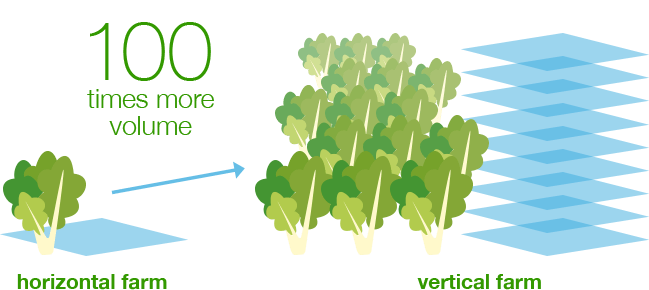
\includegraphics[width=0.7\linewidth]{hor_ver_farming}
  \caption{Vertical farming increases the volume of production per squared meter.}
  \label{fig:horizontal_vertical_farming}
\end{figure}

With these many points in favour, Indoor Vertical Farming is still not the most common farming methodology. Mostly due to the initial costs and evolving/unstable technology, farmers opt by growing their fields the traditional way. This does not mean that farmers fear technology but progress is slow, especially within the more traditional and manual labour communities. 

A farm is a place where agricultural activities take place. For organisational purposes, farms are usually split into plots which provide the first level of organisation.

\begin{figure}[htbp]
  \centering
  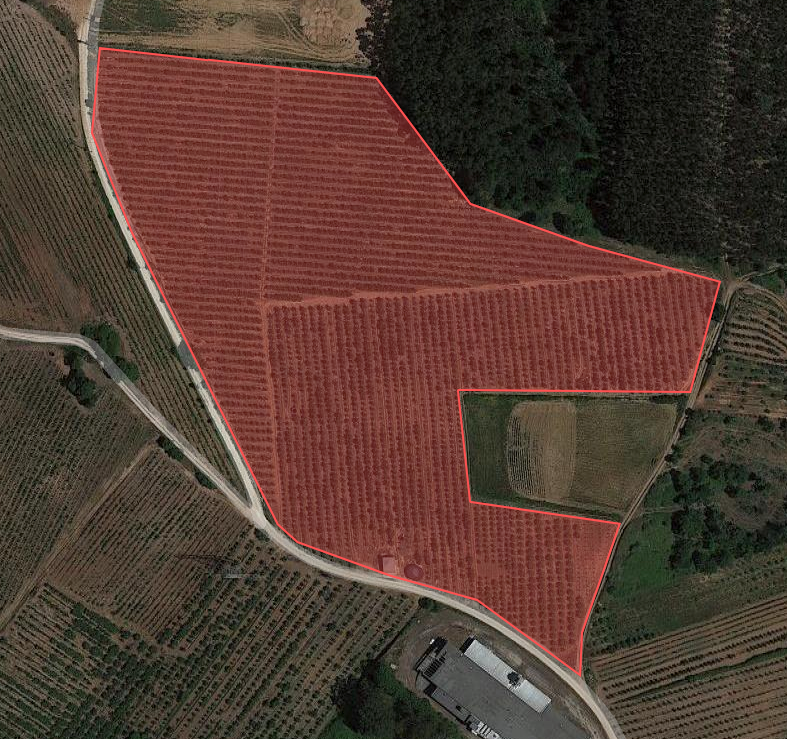
\includegraphics[width=0.5\linewidth]{field_with_plots}
  \caption{Vale Pragrança: a farming field from the FitoAgro project. Three plots are visible in the satellite image.}
  \label{fig:field_with_plots}
\end{figure}

For a plot, a single type of plant is installed. During this dissertation, the focus will be on Royal Gala Apple (Malus pumila) and Pear "Rocha" (Pyrus communis) crops.

\begin{figure}[htbp]
  \centering
  \subcaptionbox{\textit{Malus "Royal Gala"}\label{fig:royal_gala}}%
    {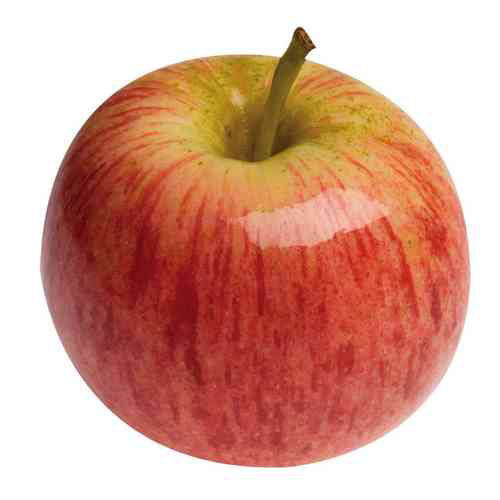
\includegraphics[width=0.5\linewidth]{royal_gala}}%
  \hfill  
  \subcaptionbox{\textit{Pyrus Communis "Rocha"}\label{fig:pear_rocha}}%
    {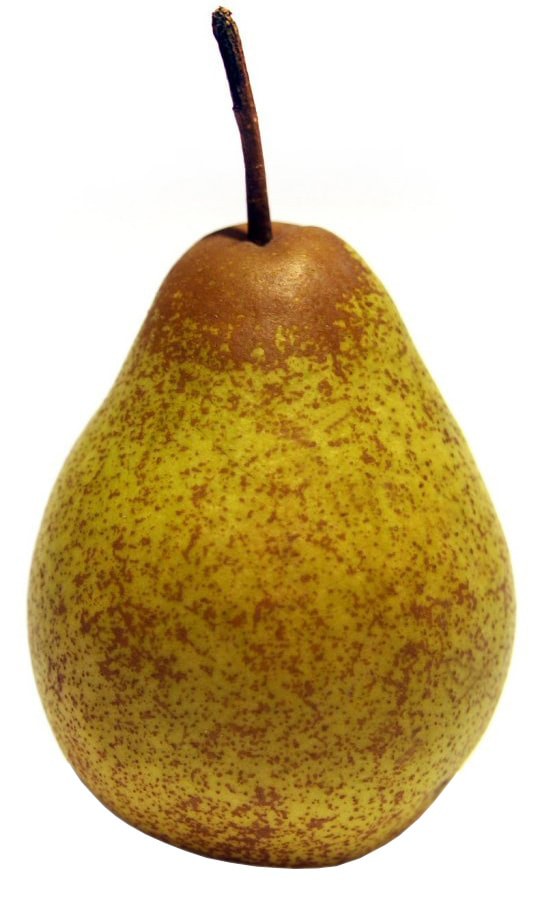
\includegraphics[width=0.4\linewidth]{pera_rocha}}%
  \caption{Crops to be monitored during this dissertation}
  \label{fig:crops_studied}
\end{figure}

\section{Spreadsheets} %%%%%%%%%%%%%%%%%%%%%%%%%%%%%%%%
\label{sec:problem_spreadsheets}

Integrated production by farmers requires certain obligations and responsibilities. Some countries have strict regulation on agriculture while others provide no guidelines for cooperation on agricultural activity. Portugal provides on the DGADR ("Direção-Geral de Agricultura e Desenvolvimento Rural") website a field notebook template for the most common plant cultures grown in Portugal.

These notebooks track the most important things happening during the production cycle: 

\begin{enumerate}
	\item Phenological Growth Stages of the crop
	\item Observations regarding the main enemies of the crop
	\item Dates of the treatments performed on the field and the phytopharmaceutical products used
	\item Production system data (pruning, watering, fertilising and harvesting)
\end{enumerate}

Field notebooks were once used on paper, but nowadays, since teams take turns working on the fields, most agronomists and farmers upload their paper records to online collaborative spreadsheets. 

\subsection{Phenological Growth Stages}
\label{sec:problem_spreadsheets_phenological}

Phenology is the study of periodic plant and animal life cycle events and how these are influenced by seasonal and interannual variations in climate. In the context of this dissertation: the growth rate of a plant and how it is influenced by temperature, light and humidity. 

Precise tracking of the phenological stage of a plant is of the utmost importance since some pests, diseases and products may depend on the current stage.

Different plant species have different phenological stages. Since this work focuses on Pome tree species, namely Apple (Malus Pumila) and Pear (Pyrus Communis) trees, the respective phenological stages of growth are illustrated on \ref{fig:pheno_apple_raw} and \ref{fig:pheno_pear_raw}.

\begin{figure}[htbp]
  \centering
  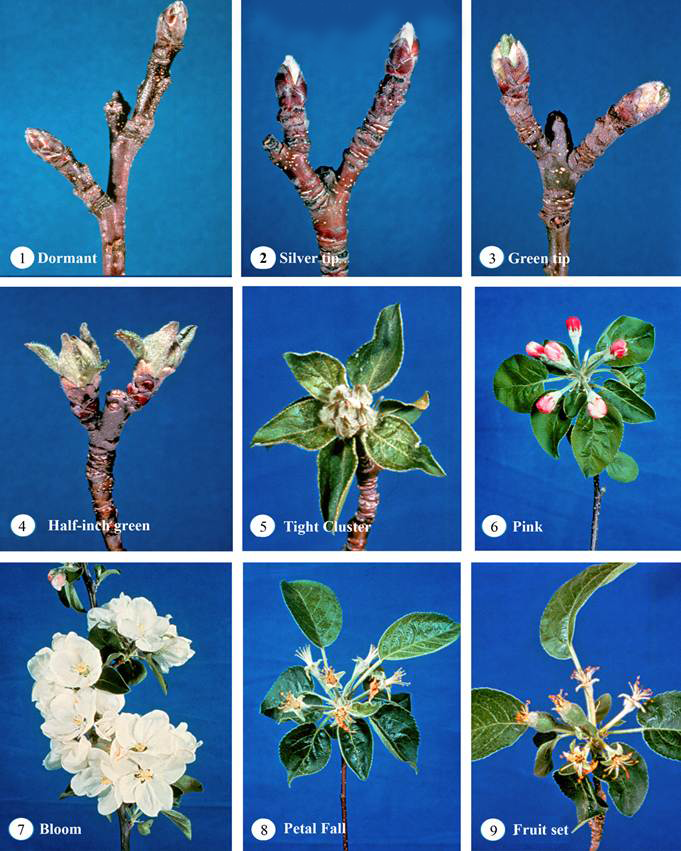
\includegraphics[width=0.7\linewidth]{pheno_apple_raw}
  \caption{Phenological Stages of Malus Pumila - by TheJentschLab \cite{TheJentschLab}}
  \label{fig:pheno_apple_raw}
\end{figure}

\begin{figure}[htbp]
  \centering
  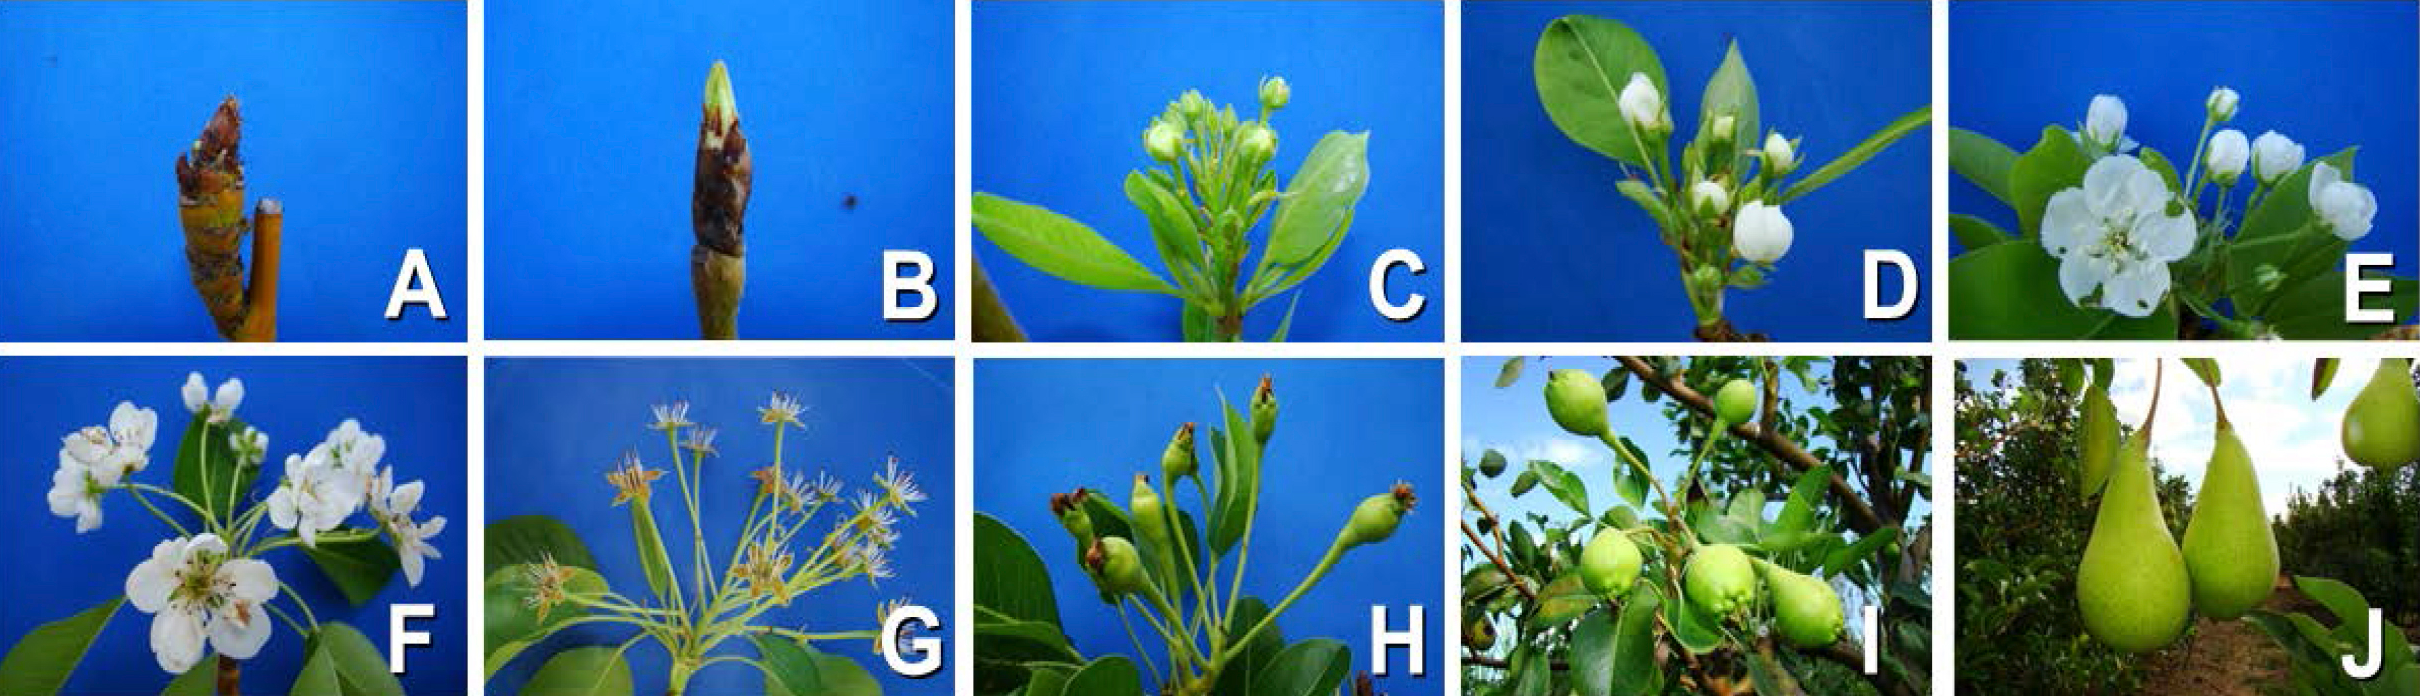
\includegraphics[width=1\linewidth]{pheno_pear_raw}
  \caption{Phenological Stages of Pyrus Communis - by TheJentschLab \cite{TheJentschLab}}
  \label{fig:pheno_pear_raw}
\end{figure}


\subsection{Enemies}
\label{sec:problem_spreadsheets_enemies}

As mentioned in \ref{sec:digital_mapping_framework}, farming fields have, by default, ideal conditions for the development of life. This attracts new species to the farming field, which usually directly impacts the economic viability of the yield. They can compromise the appearance of the product which affects the final consumer and, therefore, translates into a cut on the income of the farming company.

Enemies can be of three major types:
\begin{description}
	\item [Parasitic plants] Plants growing in non-desirable places that derive some or all of its nutritional requirement from another living plant (or from resources allocated to it)
	\item [Pests] Animal organisms that parasitise the plants.  Usually ectoparasites such as mites, insects, molluscs, vertebrates or any other life form that consumes plant tissue.
	\item [Diseases] Caused by pathogens (infectious organisms) and environmental conditions (physiological factors). Organisms that cause infectious disease can be fungi, bacteria, viruses etc.
\end{description}

Farmers register major occurrences of any of these three enemy types on the field-notebooks.

\subsection{Treatments and Control}
\label{sec:problem_spreadsheets_control}

Farmers deal with different enemies in different ways. 

\begin{description}
	\item [Herbicide] Herbicides, also commonly known as weedkillers, are chemical substances used to control unwanted plants. Non-selective herbicides kill all plant material with which they come into contact (mostly used for construction). Selective herbicide control specific weed species, while leaving the desired crop relatively unharmed.
	\item [Pesticide] Used to control animal organism life forms.
	\begin{description}
		\item [Insecticide] Insecticides are substances used to kill insects. They include ovicides and larvicides used against insect eggs and larvae, respectively.
		\item [Acaricide] For acari pests. Acari (or Acarina) are a taxon of arachnids that contains mites and ticks.
	\end{description}
	\item [Fungicide] Active substance(chemical compound) or biological organism used to kill or inhibit fungi or fungal spores (diseases).
\end{description}

\section{Pests}
\label{sec:problem_pests}

From the Fitoagro project, it was possible to sample the most harmful pests to the Royal Gala Apple and the Pear "Rocha"  Tree species.

\begin{itemize}
	\item \textit{Dasineura pyri (Bouché)} - Pear leaf-curling midge
	\item \textit{Aphanostigma pyri} - Pear phylloxera, Pear bark aphid
	\item \textit{Cydia pomonella} - Codling moth
	\item \textit{Quadraspidiotus perniciosus} - San José scale, Pernicious scale, California scale
\end{itemize}

This section \ref{sec:problem_pests} is heavily based on the Pest Encyclopedia Hyppz. Hypzz is an encyclopaedic database of 297 records describing important pests (insects, mites, rodents, nematodes, gastropods and small vertebrates) in Western Europe.

\subsection{Dasineura pyri (Bouché)}
\label{sec:problem_pests_cecidomia}

\begin{figure}[htbp]
  \centering
  \subcaptionbox{\textit{Dasineura pyri} adult drawn from a microscope setting.\label{fig:dasineura}}%
    {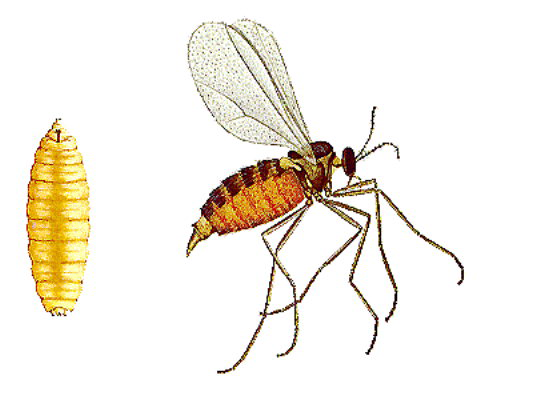
\includegraphics[width=0.55\linewidth]{dasineura}}%
  \hfill  
  \subcaptionbox{Damage on \textit{} The terminal leaves are severely distorted (arrowed).\label{fig:pear_rocha}}%
    {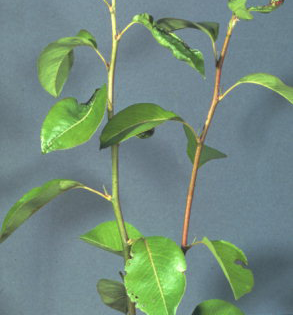
\includegraphics[width=0.42\linewidth]{dasineura_effects}}%
  \caption{\textit{Dasineura pyri} and its effects on \textit{Pyrus Communis}}
  \label{fig:dasineura_figs}
\end{figure}

Dasineura is a genus of midges in the family Cecidomyiidae. 

\subsubsection{Description}

\begin{description}
	\item [Adult] 2 to 3 mm. Black. In the female, the ovipositor is able to extend considerably (up to body length).
	\item [Eggs] Reddish.
	\item [Larva] 2 mm. Tapered at each end, pronounced tranverse segmentation, well-developed sternal spatula. Yellowish-white.
\end{description}

\subsubsection{Biology}

\begin{description}
	\item [Host plant] Pear
	\item [Adult] Very short life.
	\item [Fecundity] 30 eggs.
	\item [Eggs] Time until hatching, 3 to 4 days.
	\item [Larva] Time until pupation: 10 to 12 days
\end{description}

\subsubsection{Life Cycle}

3 to 6 generations per year. The adults appear in the spring, mate and lay eggs the same day. The female deposits the eggs on the underside of the still-furled leaf edges. The larva discharges saliva containing an auxin-related toxic substance over the leaves enabling it to feed on the cell contents. Some of the larvae pupate within the curled-up leaf, others fall to the ground, bury themselves and undergo diapause in a cocoon. Pupation begins in March.

\subsubsection{Damage}

The young leaves of attacked shoots remain curled up longitudinally. The leaf blade thickens considerably, becoming rigid and brittle. The 2nd and 3rd generations cause the greatest damage since they occur when shoot vigour and the formation of young leaves is most prolific.

\subsubsection{Monitoring}

\begin{figure}[htbp]
  \centering
  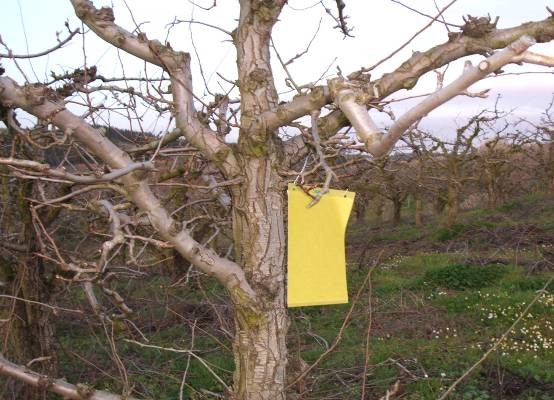
\includegraphics[width=0.7\linewidth]{dasineura_monitoring}
  \caption{Chromotropic trap made of adhesive sheet}
  \label{fig:dasineura_monitoring}
\end{figure}

Risk estimation for the Dasineura pyri pest is calculated based on the visual observation of damages on fruits, by sampling 100 sprouts in 50 trees from April to June. The economic level of attack is 15\% for saplings (young trees) and 50\% for adult trees.

Biological observations should monitor five sprouts (apples or pears) in 20 trees spread across the field. Observations should happen weekly between sprouting and late July.

Adult captures are usually performed with chromotropic traps as seen in figure \ref{fig:dasineura_monitoring}.  The chromotropic traps are adhesive sheets made of stiff and resistant plastic, with its two sides covered by a high-quality dry glue, water resistant, with no toxic substances and high-temperatures resistant.

\subsection{Aphanostigma pyri - Pear phylloxera}
\label{sec:problem_pests_filoxera}

\begin{figure}[htbp]
  \centering
  \subcaptionbox{\textit{Aphanostigma pyri} specimen.\label{fig:aphanostigma}}%
    {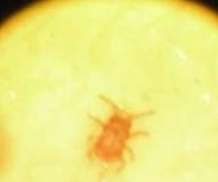
\includegraphics[width=0.45\linewidth]{aphanostigma}}%
  \hfill
  \subcaptionbox{Colony in the spring. Females, eggs and young nymphs.\label{fig:aphanostigma_effects}}%
    {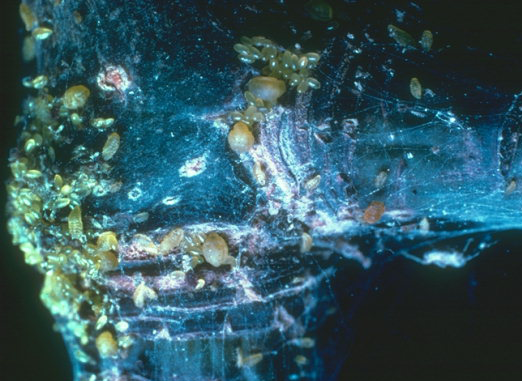
\includegraphics[width=0.5\linewidth]{aphanostigma_effects}}%
  \caption{\textit{Aphanostigma pyri} specimen and colony}
  \label{fig:dasineura_figs}
\end{figure}

\subsubsection{Description}

The insect is a holocyclic phylloxerid with the following biological phases:
\begin{itemize}
	\item Virginiparae and sexuparous females of piriform shape, whitish or lemon yellow with a length of 0.8-1.0 mm with well developed piercing-sucking mouthparts.
	\item Smaller (about 0.5 mm) sexuales with no mouthparts, ovoid in form.
	\item Eggs of sexuparae of a yellow green colour.
	\item Winter eggs with a diameter of 0.3 mm.
\end{itemize}

\subsubsection{Biology}

 The host is pear. Most attacked cultivars are, in Portugal, Passe Crassane, Comice, Douillard and Rocha. Other varieties are also attacked but less seriously.

\subsubsection{Life Cycle}

The complete life-cycle is as follows: virginiparous females hatch from winter eggs giving rise to several generations of identical types of female. Sexuparae appear in September. These lay male and female eggs from which, in the autumn, the sexuales emerge. After mating these lay the winter eggs.

In Portugal it is not known if the complete life-cycle, as described, occurs every year. No winter eggs have been found in certain areas. The overwintering form being then the parthenogenetic female.

\subsubsection{Damage}
In August sexuparae take shelter in the apical growth especially on those of late varieties where this area does not close completely. The feeding activity of these females produces large black areas on the fruit.

These black areas will appear, sometimes on other parts of the fruit, for instance where a leaf or fruit touches another fruit. Occasionally the black lesions will occur in the peduncular groove.

The commercial value of the damaged fruits will be severely reduced, often by 50\% to 60\%. The damage may occur:
\begin{itemize}
	\item During the maturation period, on the tree.
	\item During the cold storage together with the lesions caused by storage rots.
\end{itemize}

\subsubsection{Monitoring}

\begin{figure}[htbp]
  \centering
  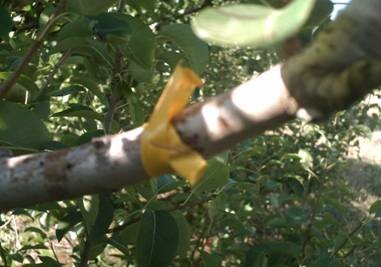
\includegraphics[width=0.7\linewidth]{aphanostigma_monitoring_1}
  \caption{WURTH Adhesive tape in a branch}
  \label{fig:aphanostigma_monitoring}
\end{figure}

\begin{figure}[htbp]
  \centering
  \subcaptionbox{\textit{Aphanostigma pyri} trap made of \textit{WURTH} adhesive tape.\label{fig:aphanostigma_monitoring_2}}%
    {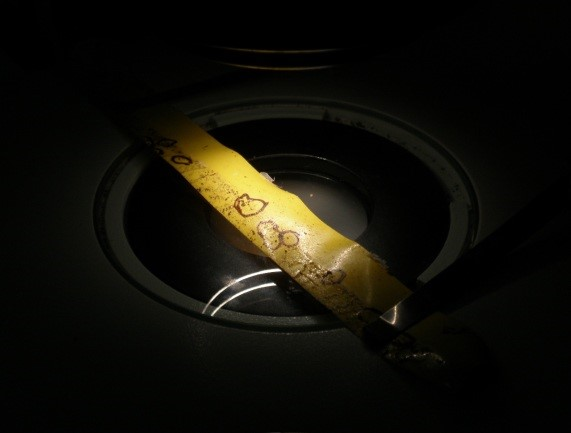
\includegraphics[width=0.47\linewidth]{aphanostigma_monitoring_2}}%
  \hfill
  \subcaptionbox{Trap under analysis in lab. \label{fig:aphanostigma_monitoring_3}}%
    {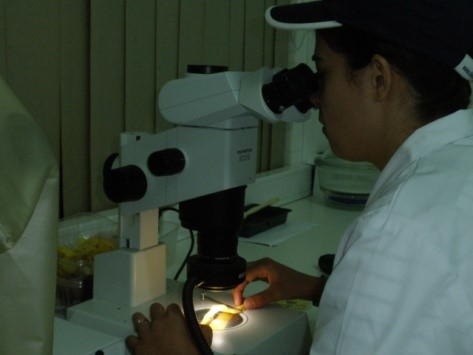
\includegraphics[width=0.47\linewidth]{aphanostigma_monitoring_3}}%
  \caption{\textit{Aphanostigma pyri} trap being analysed in laboratory.}
  \label{fig:cydia_figs}
\end{figure}

Since different life cycles have been found, biological observations should provide risk estimations but, also answer some questions on how exactly how the species behaves, requirement for the FitoAgro project.

\begin{itemize}
	\item First appearance of the virginiparous females
	\item Migration to the fruit
	\item Descent from the fruit to the tree trunk
\end{itemize}

These moments above present key changes in the life cycle of this species, so they will be tracked by registering the presence of specimens in the tree trunk, branches, twigs and fruit.

The observation method is, to the say the least, interestic. WURTH Adhesive tape is used along with flannel patches, vaseline and plastic sheets. 

\begin{enumerate}
	\item Adhesive tape on trunk and two branches (opposing directions)
	\item Adhesive tape on four twigs with fruit.
	\item Fruit monitoring before harvest. Three fruits from random trees, plus three fruits from trees that were tracked during that season.
	\item Fruit monitoring during harvest - Five fruits from each of ten random trees, plus five fruits from each of ten tree that were tracked during that season. Cut fruit through the middle to test presence of specimens.
	\item Flannel patches after harvesting until next season. By april, apply vaseline on the flannel patches.
\end{enumerate}


\subsection{Cydia Pomonella - Codling moth}

\begin{figure}[htbp]
  \centering
  \subcaptionbox{\textit{Cydia Pomonella} adult.\label{fig:cydia}}%
    {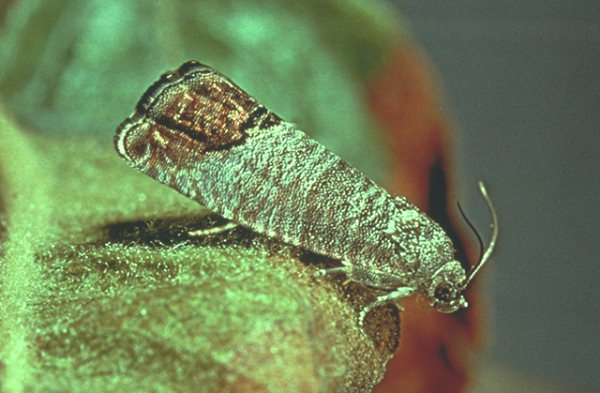
\includegraphics[width=0.5\linewidth]{cydia}}%
  \hfill
  \subcaptionbox{Second instar larva. Devouring the pips in the carpellary cavity.\label{fig:cydia_effects}}%
    {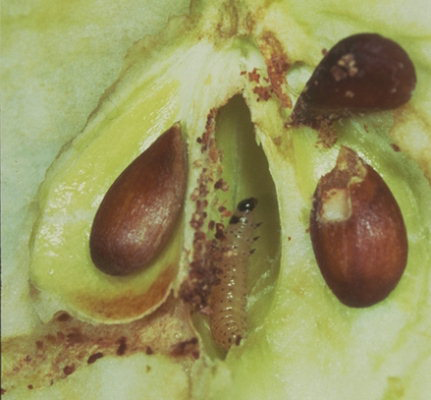
\includegraphics[width=0.4\linewidth]{cydia_effects}}%
  \caption{\textit{Cydia pomonella} adult and larva phases.}
  \label{fig:cydia_figs}
\end{figure}

\subsubsection{Description}

\begin{description}
	\item [Adult] Wingspan 16 to 19 mm. Very obvious and characteristic brown oval marking, surrounded by 2 shiny golden brown lines, tending towards the bronze, on the grey fore wings. Hind wings reddish brown, delicately ciliated.
	\item [Eggs] 1 mm diameter. Circular, flattened, slightly swollen in the middle. Laid singly on the upper side of the leaf, on the fruit or twig. Milky-white at first, then, a few days later, with presence of a reddish ring at the periphery.
	\item [Larva] 16 to 20 mm. Head dark brown; body pale pink to reddish. Abdominal prolegs, anal prolegs.
	\item [Pupa] 10 to 12 mm. Yellow-brown to dark brown. Occuring in silky cocoon.
\end{description}

\subsubsection{Biology}

\begin{description}
	\item [Host plants] Apricot, quince, walnut, pear, apple and sometimes peach and plum.
	\item [Adult] Medium longevity, 15 to 18 days. Active during the day at temperatures of > 15°C.
	\item [Fecundity] 30 to 50 eggs, on average.
	\item [Eggs] Time until hatching, 18 days at 15°C, and 6 at 25°C.
	\item [Larva] Developmental duration, 20 to 30 days.
	\item [Pupa] Developmental duration, 20 to 28 days.
\end{description}

\subsubsection{Life Cycle}

The eggs hatch at the end of May. The caterpillar first undergoes a so-called "wandering stage" (2 to 5 days). After a couple of exploratory bites, it penetrates a fruit where a second fruit or a leaf is touching, or at the stalk or stalk-eye. When development is completed, it leaves the fruit and weaves a cocoon in a sheltered spot. From then onwards, two developmental routes are possible: it will either pupate and give rise to a 2nd-generation of moth, or enter diapause. The caterpillars that become fully fed from August to October all enter diapause. They overwinter in cocoons hidden in cracks in the tree-trunk or in a natural shelter on the soil.

Pupation in April. The adults emerge at the end of April, beginning of May. They mate and lay the eggs on leaves, twigs, or young fruits.

\subsubsection{Damage}

On pomaceous fruit, around the entrance hole made by the young larva, a gnawed area, followed by a spiral gallery leading down to the pips which the caterpillar also eats. On walnuts, the caterpillar burrows through the husk to the kernel; when the latter hardens, it leaves by the hilum or remains in the husk. The bite marks on the damaged fruit makes them impossible to sell. Damaged fruit drops prematurely.
Late or seasonal varieties of pear are not very susceptible to the 1st generation because their epidermis is hard.

\subsubsection{Monitoring}

Biological observations should monitor fifty fruits per tree on a total of twenty trees spread randomly across the farming field. Observations should occur once per week. 

Risk estimation for the Cydia pomonella pest is calculated based on the visual observation of damages on fruits. The attack percentage is the percentage of attacked fruits in a total sample of one thousand fruits. 

Capturing is achieved by releasing sexual pheromones inside a trap as seen in figure \ref{fig:cydia_monitoring}. Number of caught specimens should be recorded, the trap cleaned and set up for the next week.


\begin{figure}[htbp]
  \centering
  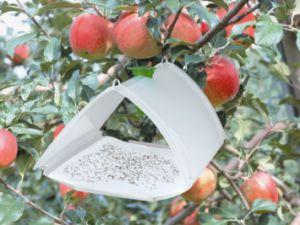
\includegraphics[width=0.7\linewidth]{cydia_monitoring}
  \caption{Sexual pheromone trap for \textit{Cydia Pomonella}}
  \label{fig:cydia_monitoring}
\end{figure}

\subsection{Quadraspidiotus perniciosus}

\begin{figure}[htbp]
  \centering
  \subcaptionbox{\textit{Quadraspidiotus perniciosus} male and female individuals. The scale of the female was turned upside down to show the colour of the body of the female. Young nymphs can be seen (arrowed).\label{fig:quadraspidiotus}}%
    {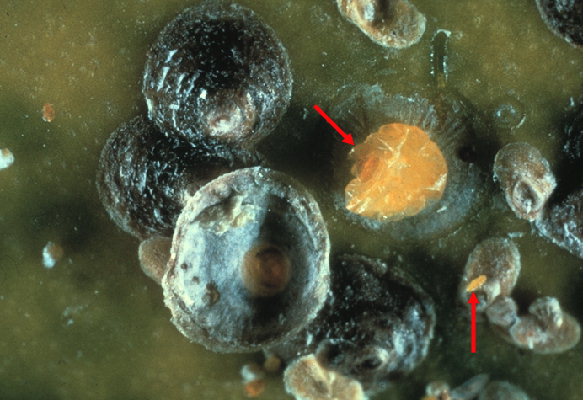
\includegraphics[width=0.47\linewidth]{quadraspidiotus}}%
  \hfill
  \subcaptionbox{Damage on pear. The change in colour of the epidermis is due to the presence of scale insects. Figure from Hyppz \cite{AlainFraval} \label{fig:quadraspidiotus_effects}}%
    {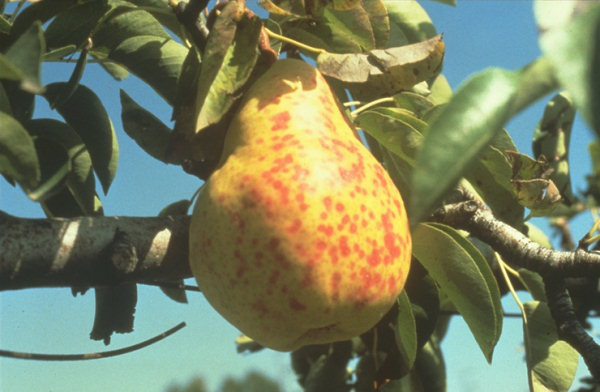
\includegraphics[width=0.47\linewidth]{quadraspidiotus_effects}}%
  \caption{\textit{Quadraspidiotus perniciosus} male, female and effects on product.}
  \label{fig:quadraspidiotus_figs}
\end{figure}

\subsubsection{Description}

\begin{description}
	\item [Adult] Female apterous, pear-shaped, flattened, fixed to the plant and hidden under a detachable scale. Scale circular, dark grey, about 2 mm across. Males provided with a pair of wings.
	\item [Nymph] Young nymph mobile, yellow, provided with 3 pairs of short legs. Once fixed, secretes a white scale which becomes grey and finally black.
\end{description}

\subsubsection{Biology}

Also know as Cochonilha, \textit{Quadraspidiotus perniciosus} is very polyphagous and develops on more than 150 species of host, especially on apple, pear, plum, peach, cherry, currant, black currant.

Nymphs overwinter during the 1st instar in a state of diapause. After moulting twice (in March and May), they emerge either as males or females. Females are viviparous and each produces 8-10 nymphs per day from late May onwards, the egg-laying period spreading over 6 weeks. The average number of nymphs produced on a favorable host plant is 400.

Nymphs are at first mobile and then settle down by inserting their stylets into plant cells. They produce encrustations on twigs, branches and sometimes on leaves and fruits.

\subsubsection{Life Cycle}

There are 2-4 generations depending on the region. As soon as winter approaches, first generation nymphs enter a state of diapause. Very young and second-generation nymphs as well as adults, die.

\subsubsection{Damage}

Feed by these insects, when they inject toxic saliva, leads to a distortion of plant tissue, the premature dropping of leaves and the discoloration of the fruits' epidermis as well as the decline of affected twigs and branches.
A specific parasite of this pest, Prospaltella perniciosi, has been introduced in some studies to fight against this scale insect.

\subsubsection{Monitoring}

Risk estimation for the Quadraspidiotus perniciosus pest is calculated based on the visual observation of branches and twigs. Percentage of attacked fruits in a total sample of one hundred fruits is the attack percentage. 

Biological observations are performed with sticky pads (seen in figure \ref{fig:quadraspidiotus_monitoring}) and should monitor five twigs per tree on a total of twenty trees spread randomly across the farming field. Observations should occur once per week by registering whether the twigs show symptoms of the insect or not. After renewal of the traps, these are sent to laboratory for species determination and counting.


\begin{figure}[htbp]
  \centering
  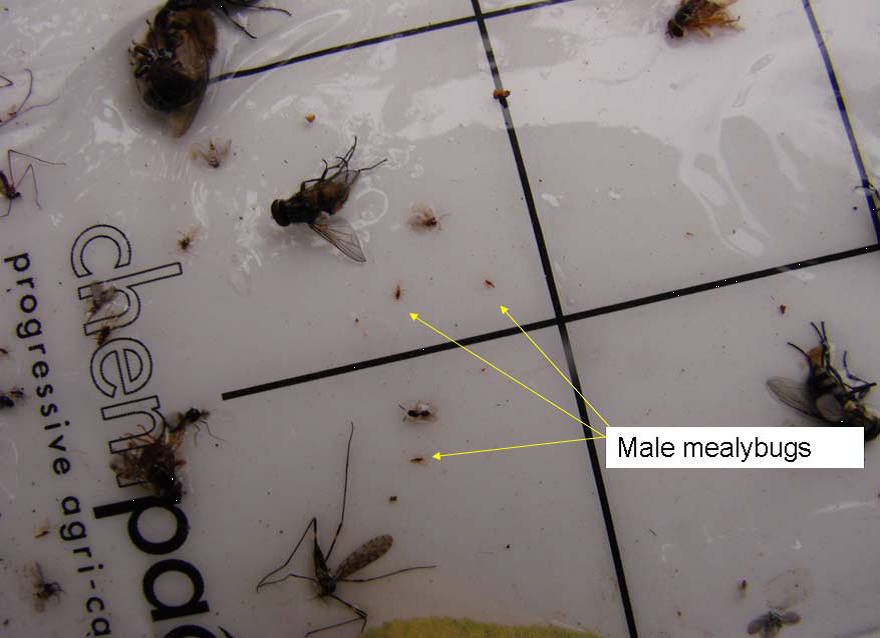
\includegraphics[width=0.7\linewidth]{quadraspidiotus_monitoring}
  \caption{Sampling of \textit{Quadraspidiotus perniciosus} males on a sticky pad.}
  \label{fig:quadraspidiotus_monitoring}
\end{figure}

\section{Data Collection}
\label{sec:problem_data_collection}

Most of the farmers and agronomists have worked in the very same fields their whole life so they know where specific events happen: the spots with less solar exposure, the irrigation defects and details, the places where water leaks, the spots with pest occurrences, the phenological cycles, the history of the field, etc. Mentally or using non-appropriate registering methodologies, they track the field variables without a proper tool.

As agricultural teams grow bigger, some information is registered to be consulted by all team members (or to keep an history). But even then, data is manually added to a spreadsheet, being Google drive the common sharing pattern among the "more advanced" cooperatives and farming companies (information from a FitoAgro project meeting).

Processing all this information requires precise and normalized inputs. This will be the main focus of this dissertation: Gathering the available data from the field to the server in an effortless and consistent way.

Even if out of the scope of this work, it is studied mostly in the state of the art, how it would be possible to fully automate the biological counting and analysis of the known enemy species by crop. Since this presents a significant problem by itself (a device that counts and analysis automatically the pests per tree that needs low to no maintenance), pseudo-automated data-collection is the closest path to ideal data-collection. Pseudo-automated data collection meaning that humans will play a key role in the registering of occurrences but some extra processing should be done in the background to ease out the task for the user.

%!TEX root = ../template.tex
%%%%%%%%%%%%%%%%%%%%%%%%%%%%%%%%%%%%%%%%%%%%%%%%%%%%%%%%%%%%%%%%%%%%
%% chapter3.tex
%% NOVA thesis document file
%%
%% Chapter with a short laext tutorial and examples
%%%%%%%%%%%%%%%%%%%%%%%%%%%%%%%%%%%%%%%%%%%%%%%%%%%%%%%%%%%%%%%%%%%%
\chapter{State of the Art}
\label{cha:state_of_the_art}

This Chapter aims at detailing data sources in the farming field, previous works done in this field of study, their pros and cons, limitations and viability in the FitoAgro project.

\section{Data from the field} % (fold)
\label{sec:state_of_the_art_data}


Collecting data from field and building a complete digital model of the plot is not an easy task. Several variables come into play and problems such as connectivity, low to none maintenance and cost of the equipment arise. These requirements may condition the amount georeferenced data-sources, their efficiency, resolution, autonomy, etc.

Revisiting the methodology of Precision-Agriculture, data-collection is probably the most important step in this 4-step process. In order to be able to calculate pest and disease regional economic risk levels, weather information needs to be available for indiviual fields(shapes). Hopefully, in the future, measures from different fields can be analised together in a continuous mesh including several fields as described in \cite{Ojha2015}. Different sampling points have to be spread across the region of study in order to build a map. This is not directly helpful to the farmer, since he mainly cares about his fields, but may help to better understand the behaviour of such pest species.

\subsection{Satellite Imagery}
\label{sec:satellite_imagery}

Satellite imagery is slowly becoming accessible for public use. While free satellites provide imagery with low temporal and geographic resolutions, paid services (though costly) provide very high resolutions. Multi-spectral imagery provides raw data that can be turned into temperatures, Normalized Difference Vegetation Index (NDVI), Moisture and Soil maps with resolutions up to 0.41m.

Satellite sensors deliver 16-Bit 4-Band (B,G,R,N) or 8-Band (C,B,G,Y,R,RE,N,N2) Multispectral pixel resolutions from 1.2m to 5m. Pansharpened vegetation indices can be delivered with a resolution of 30cm, 40cm or 50cm, providing greater details for analysis. 

The Sentinel-2 Satellite sensors acquires 10m 4-band (BGRN) Multispectral, 20m 4-band RedEdge and 2-band Short Wave InfraRed and 60m 3-band Coastal Aerosol, Water Vapour and SWIR Cirrus Imagery providing a choice for a good selection to search for cloud free Imagery for the Area Of Interest (AOI). This Imagery is very suitable to deliver 10m resolution NDVI or other vegetation index Imagery and moisture maps in KMZ format. Because the Sentinel-2 Satellite Imagery, provided by the European Space Agency (ESA), can be downloaded for free and requires only vegetation and soil index image processing, providing a cost effective Ag solution, covering large areas around the globe, were 10m resolution is acceptable or desired due to limited financial resources.

The satellites in the SENTINEL-2 constellation will provide a revisit time of 5 days at the equator in cloud-free conditions. The fees for Sentinel-2 produced vegetation index Imagery (NDVI, TSAVI etc.) and moisture maps are starting at US \$ 0.20\/ Ac or US \$ 0.49/ Ha for a combination of 2 vegetation indices and 1 moisture map, with a minimum commitment of 1,000 Ac or 405 Ha and 2 months of service, including the delivery of up to six (6) Sentinel-2 scenes in Natural Color and Color InfraRed (CIR), vegetation index scenes in GeoTIFF, IMG or KMZ format.

The agriculture, forestry and environmental industries have been using the standard NDVI index for many years but with the availability of hyperspectral sensors and high resolution Satellite sensors, such as WorldView-2 and WorldView-3, utilizing an expanded Multispectral reflectance range, Satellite imagery can provide a variety of vegetation indices to filter the correct band combinations for vegetation, soil and environmental analysis to support crop management.

\begin{figure}[htbp]
  \centering
  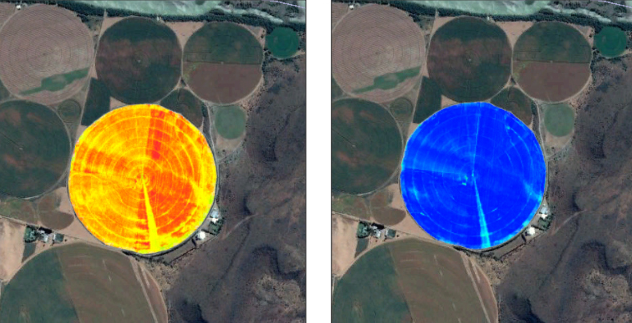
\includegraphics[width=0.9\linewidth]{worldview-2-moisture-map-ndvi}
  \caption{WorldView-2 NDVI Index (left) and Moisture Map (right) - South Africa}
  \label{fig:worldview-2-moisture-map-ndvi}
\end{figure}


WorldView-3 Satellite sensors collect in addition to the standard Panchromatic and Multispectral bands, eight-band short-wave infrared(SWIR) and 12 CAVIS imagery.\\\mbox{WorldView-3} is the first multi-payload, super-spectral, high-resolution commercial satellite sensor operating at an altitude of 617 km. WorldView-3 satellite provides 31 cm panchromatic resolution, 1.24 m multispectral resolution, 3.7 m short wave infrared resolution (SWIR) and 30 m CAVIS resolution. The satellite has an average revisit time of <1 day and is capable of collecting up to 680,000 km2 per day.

In the past, a known limitation of satellite use were clouds. In cloudy days, the area under analysis could be covered in clouds, breaking line-of-sight between the satellite and a specific land location, resulting in no readings during that portion of time. Since the revisit times were usually > 1 day (i.e. 1 reading per day), this would mean that there would be days without any readings.

Biological readings from multispectral GIS(Geographic Information System) for each of the plants is still not possible. Some recent studies have shown progress in using SWIR for optical remote detection but, using satellite imagery, the only part of the tree visible is the crown (composed by leaves, twigs and branches). The resolution of 0.31 (max resolution of the WorldView-3), even if generally considered good, is not good enough to track these micro organisms. Example of SWIR for canopy assesement in figure \ref{fig:managed-canopy-web}.

\begin{figure}[htbp]
  \centering
  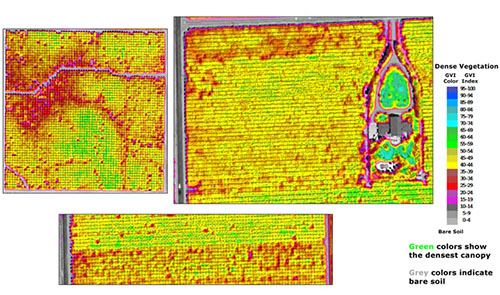
\includegraphics[width=0.9\linewidth]{managed-canopy-web}
  \caption{Managed Canopy Assessment (tree chrowns). Soils(top left), Health (top right) and Irrigation(bottom). Image from Worldview-3.}
  \label{fig:managed-canopy-web}
\end{figure}

Analysis drawn from this data-source are essentially growth indicators by vegetation indices (from reflectance and Chlorophyll), soil temperatures from shortwave infrared and irrigation if using the WorldView-3 SWIR.

In sum, there is a tradeoff between resolution/features and pricing. For agricultural use, there are no tight requirements in revisit times (temporal resolution) nor image resolution but the features from Worldview-3 in terms of Infrared analysis are revolutionary. While Short-Wave Infrared (SWIR) bands add spectral coverage to the invisible range, providing ground-breaking analysis of the land surface, CAVIS (stands for Clouds,  Aerosols, Water Vapor, Ice and Snow) corrects for the inconsistencies caused by certain conditions, offering standardized imagery no matter where or when the data was captured.

\subsection{Weather Stations}
\label{sec:weather_stations}

Weather stations provide measurements from a single location: the station location. In theory, while providing accurate readings, weather stations have initial costs and/or fixed costs (depending on the brand of the station) and maintenance is scarce due to their remote locations. In reality, most of the fields that have weather stations, their sensors are not accurate (require calibration) or completely not working.

Weather stations networks are publicly available for free but with minor issues. Data access is somewhat limited: Measurements are not available through API, and the exporting capabilities are somewhat hard to incorporate into the system

The FitoAgro project has facilitated weather stations already operating, so, to drive costs down and speed up developments on the data collection process, weather stations will be used as a starting point (with the possibility of extending and interpolation using Satellite imagery as described in \ref{sec:satellite_imagery}. Some weather stations already incorporate soil sensing capabilities, but this is obviously dependant on the brand of the equipment.

\begin{figure}[htbp]
  \centering
  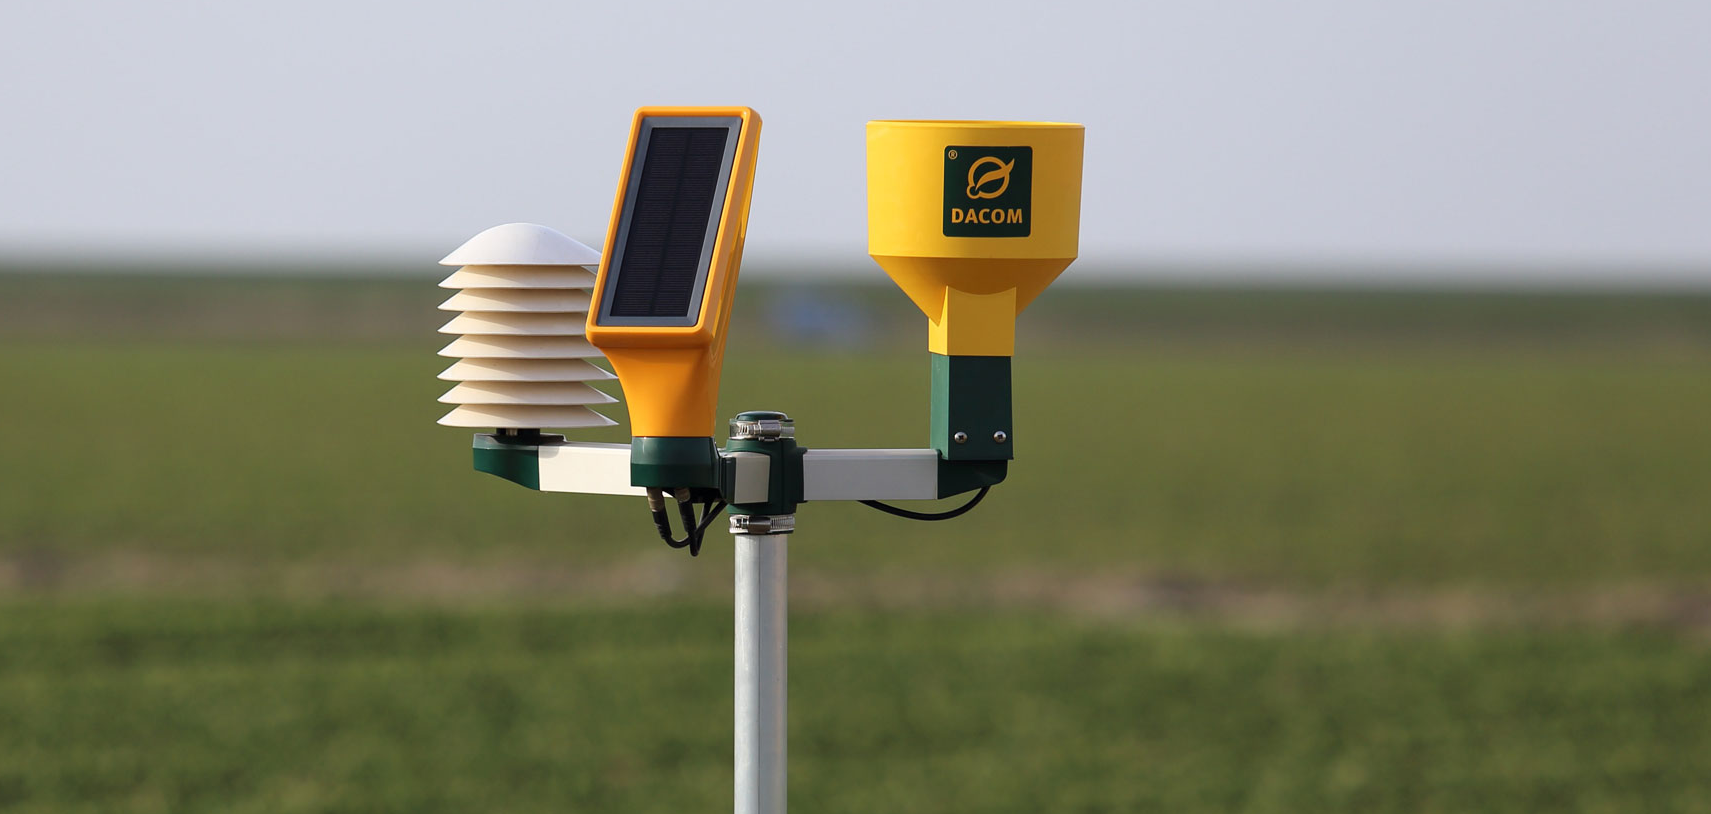
\includegraphics[width=0.7\linewidth]{weather_station}
  \caption{Simple weather station with 3 sensors: temperature, relative air humidity and rain gauge.}
  \label{fig:weather_station}
\end{figure}

The single point measurement is a problem itself: it does not provide enough data to map to the field. Two opposing corners of the same farming field will inherit the same weather and soil information since there is no way to provide better granularity using a single weather station. For the work developed in this dissertation, it is assumed that the weather variations throughout a single farming field are negligible (weather measurements not human influenced, i.e. irrigation affecting soil moisture).

In the end, the variables that we are able to gather from weather stations with minimum accuracy within the project context are:

\begin{itemize}
	\item Relative Air Temperature
	\item Relative Air Humidity
	\item Wind speed and direction
	\item Solar radiation
	\item Liquid precipitation (pluviometer or rain gauge)
	\item Atmospheric pressure
	\item Humectation (moisture)
	\item Evapotranspiration (ETo)
\end{itemize}

\subsection{Soil Analysis}
\label{sec:soil_station}

Because of on-going research and general interest in soil health and sustainability growing every year, monitoring soil in a more substantial and quantifiable way is becoming more important. In the past, monitoring the soil meant going out and physically handling the soil, taking samples, and comparing what was found to existing knowledge banks of soil information.

While nothing will replace actually going out and handling the soil for basic information, today's technology makes it possible to remotely monitor soil and track parameters that simply can't be easily or quickly measured by hand. Soil probes are now extremely accurate and offer an unparalleled look at what is going on below the surface. Giving instantaneous information on soil moisture content, salinity, temperature, and more, soil sensors are an important tool for farmers.

In order for any soil probe to work, no matter the type, it must make contact with the soil. The most accurate soil probe will be fully surrounded by the soil, with no gaps or air holes between the probe and the soil. The probe then sends electrical signals into the soil, measures the responses, and relays this information to a data collection device known as a data logger.

Common soil monitoring stations will incorporate several soil probes, at different depths. The idea is that by combining the measurements from each of the probes, it is possible to track water deployed by the irrigation system. When water is applied to this soil, these sensors reveal data about how quickly the water penetrates down through the soil, if it stagnates are certain depths and other related information. By knowing how long it takes for the water to reach the root zone, the farmer can adjust his irrigation schedule accordingly. 

Soil sensing is still not widely used due to the number, therefore cost, of sensors required to actually draw conclusions from the water management of a field.


\subsection{Enemy tracking}

Certain crops have well known enemies. In this dissertation, regarding enemies, the focus will be on pests. Unlike the previously mentioned sensing systems, pest tracking heavily relies on human interaction. Full automation of enemy tracking, even if possible, is hard to achieve and totally out of the scope of this dissertation. 

 Different pests have different tracking methodologies as described in chapter \ref{sec:problem_pests}. 

To successfully interpret these biological measurements, an appropriate interface for registering these metrics has to be created. To replace Google Drive as a platform for data registry, a custom mobile application will be created for the FitoAgro project, applying the methodology defined in this dissertation. 

The development of a mobile application for farmers and agronomists to use is of the utmost importance to request data from the database system or the results from our pest models and allow them to manually submit interactions such as plant treatments, enemy observations and plant phenological stages.

Proper geovisualization can enhance and ease out the data collection process by providing the user with a clear map of the farming field: the state of each of the present pests, upcoming events, recommended trees to track, problematic spots etc.

\begin{figure}[htbp]
  \centering
  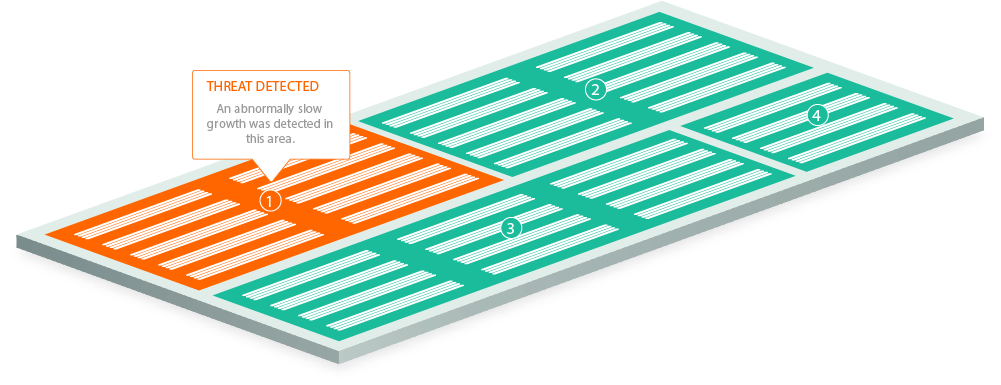
\includegraphics[width=1\linewidth]{vis_pers_lowlevel}
  \caption{Visualization work for the FitoAgro project under development.}
  \label{fig:vis_pers_lowlevel}
\end{figure}

More on the application in chapter \ref{sec:mobile_web_app}.

\section{Mobile and Web Applications} % (fold)
\label{sec:mobile_web_app}

Mobile and Web Applications are common ways to present the user with an interface to the server.

For this chapter, we consider two different use cases for the application usage:

\begin{itemize}
	\item The farmer is performing biological observations on one of his fields.
	\item The farmer is checking the state of his field and checking evolution of the pest overtime
\end{itemize}

While both use cases imply an interface for server communication, they will, most likely, be used in different contexts.

Ideally, web applications are for desktop/laptop usage. They can be responsive(readjust for any device size) but due to mobile-specific user interactions (scroll, swipe, etc.) and different design paradigms(for the two most common mobile operating systems: Apple and Android), native applications provide the user with a better interface that fits his device perfectly by following his operating system design guidelines. These rely on higher computing power (when compared to mobile devices) and bigger screens. This allows for more complex visualizations in general. 

On the other hand, mobile devices present a way for the user to interact with the system anywhere. Portability is obviously a major concern in this dissertation since farming fields are usually in remote locations. The biological observation data collection process involves movement since many trees have to be monitored throughout the field, and therefore, a small and portable device to upload information seems to be the ideal interface.

Organisations working in disparate domains are independently discovering patterns for building software that look the same. These systems are more robust, more resilient, more flexible and better positioned to meet modern demands.

These changes are happening because application requirements have changed dramatically in recent years. Only a few years ago a large application had tens of servers, seconds of response time, hours of offline maintenance and gigabytes of data. Today applications are deployed on everything from mobile devices to cloud-based clusters running thousands of multi-core processors. Users expect millisecond response times and 100\% uptime. Data is measured in petabytes. Today's demands are simply not met by yesterday’s software architectures.

The \textit{Reactive Manifesto} presents a coherent approach to systems architecture that fulfils present requirements. Systems built as Reactive Systems are more flexible, loosely-coupled and scalable. This makes them easier to develop and amenable to change. They are significantly more tolerant of failure and when failure does occur they meet it with elegance rather than disaster. Reactive Systems are highly responsive, giving users effective interactive feedback.

In general, Reactive systems are:

\begin{description}
	\item [Responsive] The system responds in a timely manner if at all possible. Responsiveness is the cornerstone of usability and utility, but more than that, responsiveness means that problems may be detected quickly and dealt with effectively. Responsive systems focus on providing rapid and consistent response times.
	\item [Resilient] The system stays responsive in the face of failure. This applies not only to highly available, mission-critical systems — any system that is not resilient will be unresponsive after a failure. Resilience is achieved by replication, containment, isolation and delegation.
	\item [Elastic] The system stays responsive under varying workload. Reactive Systems can react to changes in the input rate by increasing or decreasing the resources allocated to service these inputs. This implies designs that have no contention points or central bottlenecks.
	\item [Message Driven] Reactive Systems rely on asynchronous message-passing to establish a boundary between components that ensures loose coupling, isolation, and location transparency.
\end{description}

\subsection{Mobile Application}

Mobile Applications can be both native or cross-platform. Native Applications are built directly for the smartphone operating system while cross-platform are designed to fit more than one operating system.

There is a tradeoff between development time and performance. While cross-platform applications save time for the development team by forking developer code to both mobile standards, specific features may come with limited support and efficiency may not be as good as a native application.

\subsubsection{Native}

A native mobile app is a smartphone application that is coded in a specific programming language, such as \emph{Objective C} for \emph{iOS} or \emph{Java} for \emph{Android} operating systems. Native mobile apps provide fast performance and a high degree of reliability. They also have access to a phone's various devices, such as its camera and address book. In addition, users can use some apps without an internet connection. However, this type of app is expensive to develop because it is tied to one type of operating system, forcing the company that creates the app to make duplicate versions that work on other platforms.

\subsubsection{Hybrid or Cross-Platform}

This type of application has cross-platform compatibility but can still access a phone’s hardware. It is developed using platforms such as \emph{Sencha}, \emph{PhoneGap} or \emph{Mosync}. These were the usual approach for small teams developing for both platforms since they cut the development time in nearly half.

\subsubsection{React Native - The Best of both worlds}

Using the usual web development methodology, React Native inherited its component-based architecture from ReactJS (The predecessor and web version of React). Making use of the usual Model-View-Controller (\emph{MVC}) development pattern, this technology presents the developer with the ability to program the application once but export auto-generated native code for all the commercial operating systems: \emph{Windows Phone}, \emph{Android} and \emph{iOS}. This seems to be the modern approach of most development teams, migrating their mobile applications to React Native. The only technology that surpases \emph{React Native} in terms of performance (even though it is a minor gain) and extensibility is directly building native applications. 

\subsection{Web Application}

Web Applications, just like mobile, serve the interface to the user so that he is able to reach the computations from the server. In this subsection, some technologies are presented, discussed and compared.

\subsubsection{React}

As previously mentioned, \emph{React} is an open-source \emph{Javascript} component-based \emph{MVC}(Model-View-Controller) architecture for \emph{frontend}, made by \emph{Facebook}. \emph{React} makes it painless to create interactive UIs. Designing simple views for each state in the application, React will efficiently update and render just the right components when data changes. With components in Javascript, React renders possible the creation of a rich mobile User Interface (\textit{UI}) from declarative components.

Since component logic is written in JavaScript instead of templates, rich data can easily be passed through the app and keep state out of the \textit{DOM} (Domain Object Model).

\subsubsection{Angular}

\emph{Angular} (commonly referred to as "Angular 2+") is a \emph{TypeScript}-based open-source front-end web application platform led by the \emph{Angular} Team at \emph{Google} and by a community of individuals and corporations. \emph{Angular} is a complete rewrite from the same team that built \emph{AngularJS}.

The main difference between \emph{Angular} and \emph{React} for the web is probably the development speed. \emph{Angular} is much easier to set up and develop on, since most frontend patterns and utilities are already built-in as modules that can be imported. 

The performance is probably inferior to \emph{React}'s due to its life cycle (a continuous loop where the application looks for changes, and re-renders needed components when doing so). This is a problem for extensive applications, fast-changing \emph{DOM}s (realtime applications) but should not present a problem in this dissertation domain.



%!TEX root = ../template.tex
%%%%%%%%%%%%%%%%%%%%%%%%%%%%%%%%%%%%%%%%%%%%%%%%%%%%%%%%%%%%%%%%%%%%
%% chapter4.tex
%% NOVA thesis document file
%%
%% Chapter with lots of dummy text
%%%%%%%%%%%%%%%%%%%%%%%%%%%%%%%%%%%%%%%%%%%%%%%%%%%%%%%%%%%%%%%%%%%%
\chapter{Approach and Planning}
\label{cha:approach_and_planning}

Since two members of the FCT-UNL institution are part of the FitoAgro project and dissertation topics shall not overlap, the server processing of this data is not mentioned in this work. Data collection is, ultimately, a server routine but also an important part of the work described in this very document. This being said, this work is being closely integrated to the work in \emph{André Malafaia}'s dissertation and the technological stack is going to be decided by both during the first days of dissertation work.

The pest monitoring protocol is going to be closely followed \textit{in situ} to sucessfully iterate the proposed framework as in an agile methodology: small development cycles should be made on the framework/applications and testing on the field as features are released. The interface will be tested directly with the users in a task-based test so see if the user is able to perform the directed task or not. 

\section{Third-Party Data Collection}

The work proposed in this document starts by collecting data from weather and soil stations. Integration with FitoAgro stations (WiseCrop \cite{wisecrop} and TerraPro \cite{terrapro}) will provide field variables. This means that, against the precision agriculture methodology refered in \ref{sec:precision_agriculture}, it will be assumed that the measurements made by a single point in the field are constant throughout the entire field (for weather and soil sensors). If some farming fields have no nearby weather stations, the possibility of combining free satellite data (low temporal and geospatial resolution) is going to be analysed.

The figure \ref{fig:vis_pers_lowlevel} shows an example of a farming field visualization with low level of detail: big areas have the same variables due to low density of sensorial devices, in most cases only 1 sensor of a type per farming field). 

\begin{figure}[htbp]
  \centering
  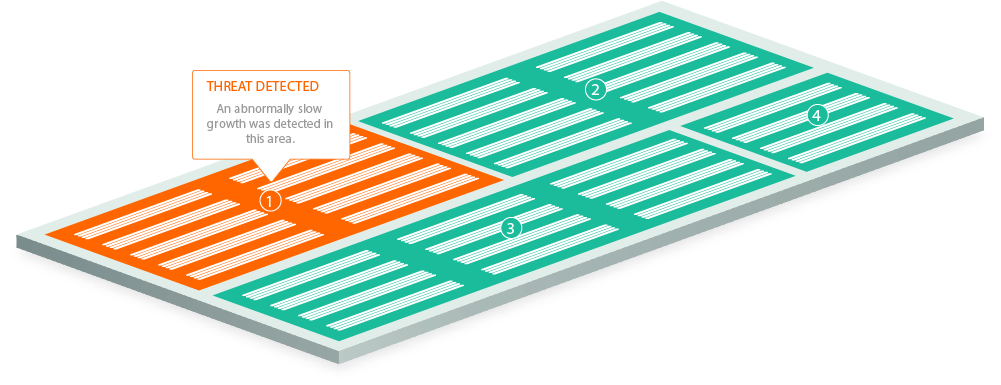
\includegraphics[width=0.8\linewidth]{vis_pers_lowlevel}
  \caption{Visualization of a farming field with a second level of detail: Plot. This assumes that 4 sensors of each type are available in the farming field represented, one for each plot.}
  \label{fig:vis_pers_lowlevel}
\end{figure}

The FitoAgro project is planned to be 4 years long. If during the first year (the time of development of the dissertation) the pest monitoring system of the FitoAgro project evolves in requisites (more spatial resolution is needed), efforts to gather more information will be made. This can mean paid satellite services (\textit{WorldView-3}) for more resolution on intra-field data collection or soil sensor meshes collecting ground information as of described in \ref{sec:soil_station}. Satellite data would mean getting crop growth levels, nutrients, soil moisture without having to install any sensors, but paying a fixed fee per hectare. Since every sensorial device has a cost, economic viability of new data sources will be fully studied.

\section{Tree-level maps for precision agriculture}

The only data that is to be collected at tree-level (measurements by tree), on this first stage of the project, are pest biological observations. Examples of tree-level visualizations for the FitoAgro project being developed can be analysed in figures \ref{fig:vis_pers_highlevel} and \ref{fig:vis_2d_highlevel}. These present the very first prototypes of the user interface design on how data is to be communicated in a user-friendly way. These are still work in progress so will, most likely, change during the course of this dissertation work.

\begin{figure}[htbp]
  \centering
  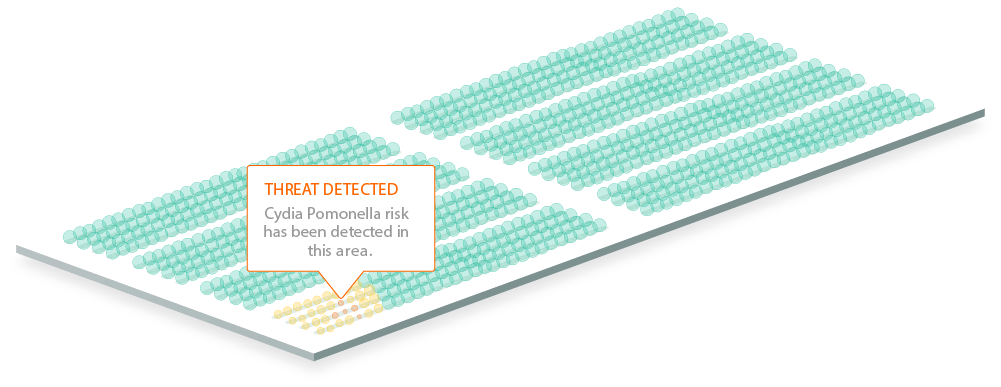
\includegraphics[width=1\linewidth]{vis_pers_highlevel}
  \caption{3D Visualization work for the FitoAgro project under development.}
  \label{fig:vis_pers_highlevel}
\end{figure}


\begin{figure}[htbp]
  \centering
  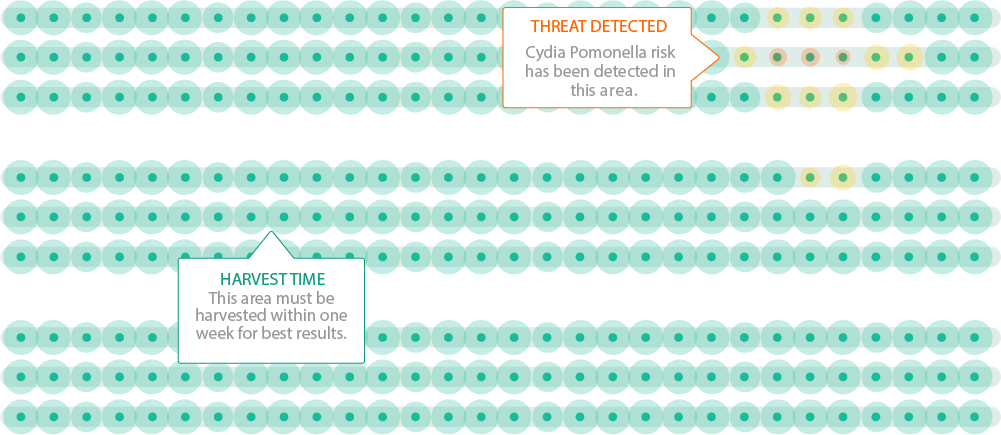
\includegraphics[width=0.7\linewidth]{vis_2d_highlevel}
  \caption{2D Visualization work for the FitoAgro project under development.}
  \label{fig:vis_2d_highlevel}
\end{figure}

These, even if prototypes, present a good starting point for both the mobile and web interfaces (assuming 2D for smaller devices and 3D for laptop/desktop, this premise will be tested with users). 

As refered in section \ref{sec:mobile_web_app}, mobile and laptop/desktop provide different interaction patterns for the user. Two very different use cases were presented and, for the analysis of the field variables, bigger screens fit more information and information with more details. This being said, the creation of a web application to support user analysis of the farming variables is of importance to ease-out the visualization process and for convenience.

\section{Web Application}

As refered in section \ref{sec:mobile_web_app}, mobile and laptop/desktop provide different interaction patterns for the user. Two very different use cases were presented and, for the analysis of the field variables, bigger screens fit more information as well as information with more details. This being said, the creation of a web application to support user analysis of the farming variables is of high importance to ease-out the visualization process and for convenience since most of the analysis work is not performed in the farming field but in the office.

The web application should present visualizations of the field on a temporal manner, attribute based maps such as risk, weather, soil temperature, wind direction, phenological stage, pest observations etc. using 2D/3D layouts depending the user preference. It shall incorporate several fields and one or more plots per field. Each plot will have data from weather, soil and biological observations as major events in the production cycle: pesticide use dates, phenological stages of the crop, water leaks etc. Like the figure \ref{vis_pers_highlevel} suggests, variables will be mapped to color, size and possible form to aggregate several data sources in the same visualization.

The end-user will play a key-role in the development of these maps since only biologists and farming professionals know the details of what is important to track and what is not. It is planned to validate these maps with partner entities of the FitoAgro project as ISA (Instituto Superior de Agronomia). As biology experts, their insight on pest life cycle tracking is important to actually draw conclusions from the data being collected. 

\section{Enemy Monitoring Mobile Application}

On enemy monitoring, an event registering interface is going to be developed to be used directly in the field when registering biological observations. When biological measurements are being performed, geolocation of the device should be taken into account to sucessfully map the measurement taken to a specific point in the field (therefore, tree being monitored).

An example of the spreadsheet currently in use by the FitoAgro project managers and farmers can be found in \ref{fig:spreadsheet} and the problems with this method are described in \ref{subsec:spreadsheets}. The plan is to design, implement and test a mobile interface for data insertion directly from the tree being monitored and collect the attached geolocation from the client mobile device.

Measurements registered from the application will have capture counts of the tracked species, in-tree location (for enemy control protocols that register several measurements from each tree - pest life cycle analysis) as shown in figure \ref{fig:spreadsheet} and their geolocation. Some server side clustering techniques will be applied to ease out collection method since the tree id is not relevant but the geolocation of that tree. As show in figure \ref{fig:k-means}, K-Means or a similar clustering algorithm can be used to reduce GPS and user positioning errors. This is the normal use case: monitored trees are decided in the season opening and stay fixed during the whole production phase. Therefore, the number of trees being tracked is always the same, and so is their position. Variance in the location of the locations registered is to be discarded.

Due to the remote location of the farming fields, internet coverage may be scarse or even inexistent. The application should support no connection to the internet by storing all the measurements in local storage and later dispatching to the server when a connection is detected. This mechanism, often described as "Offline mode", is a common pattern in recent applications and shall be incorporated in the app to be developed. Alerts in the form of push-notifications, scheduling of events and monitored tree adjustment are optional, yet planned, features. These should be available in both client applications (mobile and web).

\begin{figure}[htbp]
  \centering
  \subcaptionbox{GPS locations from measurements \label{fig:k-means_black}}%
    {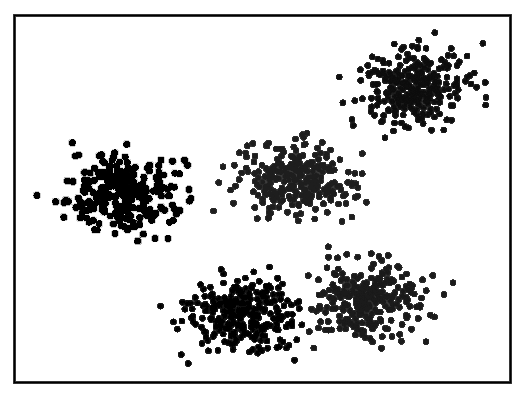
\includegraphics[width=0.5\linewidth]{k-means_black}}%
  \hfill  
  \subcaptionbox{Clustering applied to detect registered tree\label{fig:k-means}}%
    {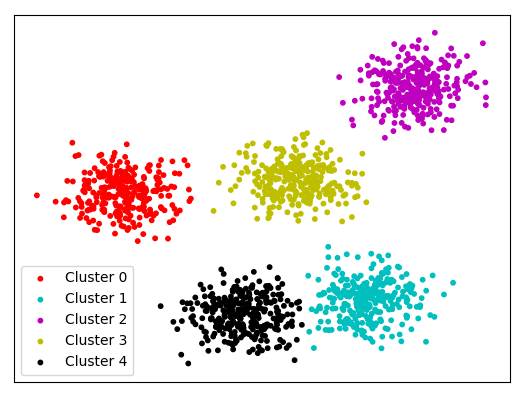
\includegraphics[width=0.5\linewidth]{k-means}}%
  \caption{K-Means algorithm applied to geolocations to reduce gps and human positioning error.}
  \label{fig:k-means-clustering}
\end{figure}

The pre-requisites for the application development have been gathered from meeting with the FitoAgro group and a shared Google Drive folder with the protocols for biological sampling as described in \ref{sec:problem_pests}.

\section{Development plan}

This section serves as description of the major tasks illustrated in \ref{fig:gantt}.

\begin{figure}[htbp]
  \centering
  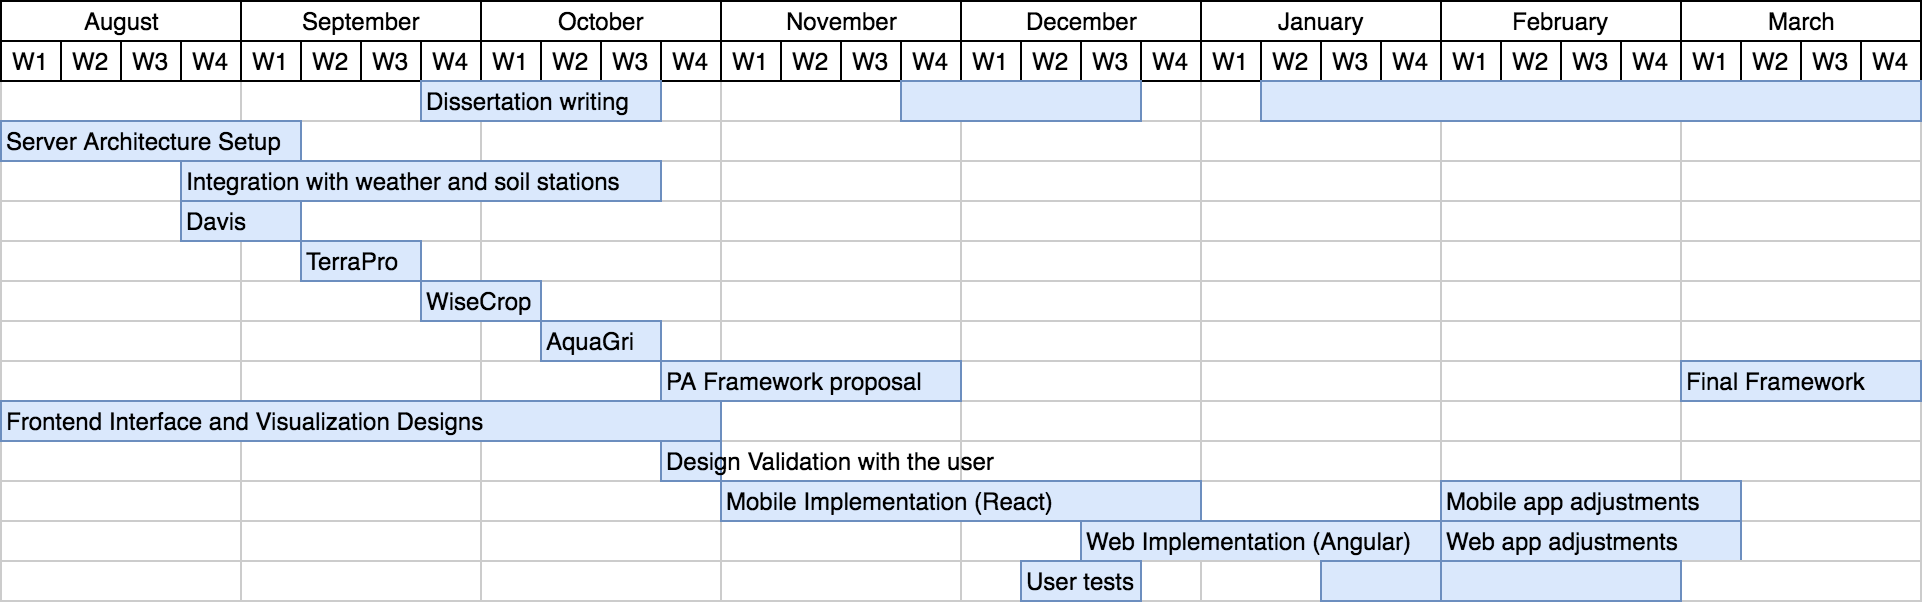
\includegraphics[width=1.5\linewidth, angle=90]{gantt}
  \caption{3D Visualization work for the FitoAgro project under development.}
  \label{fig:gantt}
\end{figure}

Server Architecture Setup - Technological stack decisions, version control, Trello board for coordination and development setup with proper tools for modern web/mobile development.

Integration with weather and soil stations - Common brands for weather and soil stations amongst the FitoAgro partners are: Davis, TerraPro, WiseCrop and AquaGri. Integration with their APIs or scrapping their content should take, two weeks per brand. 

Frontend Interface and Visualization Designs - The development of the visualization proposal showcased in \ref{fig:vis_pers_highlevel} \ref{fig:vis_2d_highlevel} will be resumed during the station integrations. This work will consider interactions, attribute based maps, screen real estate, layered organization and user experience patterns.

Mobile Application Implementation in React - Implementation of the data collection application core components: a georeferenced enemy tracking registering interface with offline usage, media management attached to biological observations and rich visualizations if the task on interface and visualization designs deems appropriate for mobile usage.

Web Application Implementation in Angular - Implementation of the extended version of the interface with full visualization screens: risk maps, soil maps, weather and pest distribution maps. These visualizations may suffer changes if requested by the FitoAgro project group or from the Agronomy experts from ISA.

Proper user testing time is allocated in the Gantt chart (figure \ref{fig:gantt}) during the final phases of mobile and web interfaces. These will consist of predefined user stories for the end-user to execute \emph{in situ}. Rates of correct execution and time taken to perform each action will be logged in order to access the user-experience of the framework developed.

%\include{Chapters/chapter7}
%\include{Chapters/appendix1}
%\include{Chapters/appendix2}
\include{Chapters/annex1}
\include{Chapters/annex2}
%!TEX root = ../template.tex
%%%%%%%%%%%%%%%%%%%%%%%%%%%%%%%%%%%%%%%%%%%%%%%%%%%%%%%%%%%%%%%%%%%%
%% glossary.tex
%% NOVA thesis document file
%%
%% Acronyms definition
%%%%%%%%%%%%%%%%%%%%%%%%%%%%%%%%%%%%%%%%%%%%%%%%%%%%%%%%%%%%%%%%%%%%
\newacronym{PA}{PA}{Precision Agriculture}
\newacronym{abbrev}{abbrev}{abbreviation of a longer text}
\newacronym{aaa}{aaa}{acornym aaa}
\newacronym{aab}{aab}{acornym aab}
\newacronym{aba}{aba}{acornym aba}
\newacronym{bbb}{bbb}{acornym bbb}
\newacronym{xpt}{xpto}{and extension of a xpto xpto xpto xpto xpto xpto xpto xpto xpto xpto xpto xpto xpto xpto xpto xpto xpto xpto xpto}

\loadglsentries[\acronymtype]{example-glossaries-acronym.tex}
\glsaddall
\include{Chapters/glossary}
\bibliography{bibliography}